%%%%%%%%%%%%%%%%%%%%%%%%%%%%%%%%%%%%%%%%%%%%%%%%%%%%%%%%%%%
%% Congratulations, you've made an excellent choice
%% of writing your Tampere University dissertation using
%% the LaTeX system. This document attempts to be
%% as complete a template as possible to let you focus
%% on the most important part: the writing itself.
%% Thus the details regarding the visual appearance
%% have already been worked out for you!
%%
%% I sincerely hope you will find this template useful
%% in completing your dissertation project. I've tried to
%% add comments (followed by the % sign) to clarify
%% the structure and purpose of some of the commands.
%% Most of the magic happens in the file
%% taudissertation.cls, which you are more than welcome
%% to take a look at. Just refrain from editing it
%% in the most crucial versions of the dissertation!
%%
%% I wish you and your dissertation project the best
%% of luck! If this template causes you trouble along
%% the way or if you've any suggestions for improving it,
%% please contact me via email at
%% 
%% ville.koljonen (at) tuni.fi.
%%
%% Yours,
%%
%% Ville Koljonen
%% 5th February 2019
%%
%% PS. This template or its associated class file don't
%% come with a warranty. The content is provided as is,
%% without even the implied promise of fitness to the
%% mentioned purpose. You, as the author of the dissertation,
%% are responsible for the entire work, including the
%% provided material. No one else is liable to you for
%% any damage inflicted on you or your thesis, were it
%% caused by using this template or not.
%%%%%%%%%%%%%%%%%%%%%%%%%%%%%%%%%%%%%%%%%%%%%%%%%%%%%%%%%%%

%%%%% INSTRUCTIONS FOR COMPILING THE DOCUMENT %%%%%
%% Overleaf: just click Recompile.
%% Terminal:
%%  1. pdflatex main.tex
%%  2. makeindex -s main.ist -t main.glg -o main.gls main.glo
%%  3. biber main
%%  4. pdflatex main.tex
%%  5. pdflatex main.tex
%% Similar sequence of commands is also required
%% in LaTeX specific editors.
%%%%%%%%%%%%%%%%%%%%%%%%%%%%%%%%%%%%%%%%%%%%%%%%%%%

%%%%% PREAMBLE %%%%%

%%%%% Document class declaration.
% The possible optional arguments are
%   finnish - thesis in Finnish (default)
%   english - thesis in English
%   numeric - citations in numeric style (default)
%   authoryear - citations in author-year style
% Example: \documentclass[english, authoryear]{tauthesis}
%          thesis in English with author-year citations
\documentclass[english]{taudissertation}

% The glossaries package throws a warning:
% No language module detected for 'finnish'.
% You can safely ignore this. All other
% warnings should be taken care of!

%%%%% Your packages.
% Before adding packages, see if they can be found
% in taudissertation.cls already. If you're not sure
% that you need a certain package, don't include it
% in the document! This can dramatically reduce
% compilation time.

\usepackage{lipsum}
\usepackage{booktabs}
\usepackage{lineno}
\usepackage{rotating}
\usepackage{array,multirow,makecell}
\usepackage[utf8]{inputenc}

%%%%% Your commands.

\usepackage{hyperref}
\def\UrlBreaks{\do\/\do-}

% Print verbatim LaTeX commands
% \newcommand{\verbcommand}[1]{\texttt{\textbackslash #1}}

%%%%% Glossary information.
\loadglsentries{tex/glossary.tex}
\makeglossaries

%%%%% Citation information.

% Use a separate .bib file to store bibliographic
% information relating to own publications.
% If you're writing a monograph, simply comment
% this out.
\addbibresource{publications/publications.bib}

% References for the dissertation.
\addbibresource{tex/references.bib}

\hypersetup{hidelinks}

\begin{document}

%%%%% FRONT MATTER %%%%%

\frontmatter

% Enter the title and a possible subtitle
% of your work along with your name here.
\title{Feasibility of remote sensing based deep learning in crop yield prediction}
\author{Petteri Nevavuori}

% Notice that this is only included for
% convenience, use the separate title page
% template to produce the final book cover pages.
\maketitle

% Write the dedication into a separate file.
% Comment out if not applicable.
\dedication{tex/dedication.tex}

% Write either 'Preface' ('Esipuhe') or
% 'Acknowledgements' ('Kiitokset').
% Write the title of this section as the first
% argument and the file name as the second.
\preface{Preface/Acknowledgements}{tex/preface.tex}

% Write the abstracts, the first one in the
% main language of the dissertation.
% Comment the other one out if not applicable
% (e.g. international students).
\abstract{tex/abstract.tex}
% \otherabstract{tex/otherabstract.tex}

% Automatically updating ToC.
\tableofcontents

% Print lists of figures, tables and programs,
% if necessary. Otherwise comment out.
% Use listings package for all code listings.
\listoffigures
\listoftables
% \lstlistoflistings

% Print a glossary of abbreviations, if necessary.
% Otherwise comment out.
\glossary


% Print the list of original publications.
% The format of the bibliographic information
% is similar to the entries in the bibliography.
% Comment out if writing a monograph.
\listofpublications
% \clearpage

%%%%% MAIN MATTER %%%%%

\mainmatter

% Write each chapter into a separate file.
% Add a \label right after the chapter name
% if you need to reference it later.

\chapter{Introduction}
\label{ch:introduction}

This doctoral dissertation studies the applicability of novel machine learning methods with remote sensing data in the context of agricultural decision support systems (DSS) in precision agriculture \cite{Bell1995} and smart farming \cite{Sundmaeker2016}. Farmers have practiced precision agriculture for ages to optimize yield productions of their fields. Sources of intra-field variability were deduced by noting and exchanging annual observations and experimenting with interventions. However, both the observations and the conclusions drawn have been more or less based on intuition, rather than on objective data. From this emerges the need for data-driven decision making, i.e. smart farming, to aid the farmers in choosing the best actions to take to optimize crop cultivation \cite{Kamilaris2017}. The application of novel deep learning techniques has been on an increasing trend for the past few years in smart farming and precision agriculture application domains \cite{VanKlompenburg2020}. One of the key reasons for this progression is the abundant availability of sensor based data in terms of ground-based soil sensors, and low-altitude unmanned aerial vehicles (UAV) and high-altitude satellite systems \cite{Wolfert2017d}. Another factor is the open-access availability of other enviromental data, such as weather and land survey data. Thus, the use of remote sensing data to extract information with machine learning models for data-driven decision making has become more common. Especially, the number of studies using deep learning techniques to perform agriculture related modelling tasks has steadily increased \cite{Kamilaris2018a}. 

Remote sensing data relevant to smart farming tends to be predominantly spatial in nature. This stems from the objects of interest - fields, forests and plots of land. Conventionally, open-access remote sensing data has been acquired from nationally operated multispectral satellite sources, such as Sentinel-2 (ESA, Paris, France) or Landsat 8 (USGS, Reston, Virginia, USA). Satellite data, while spatial, is also temporal due to regular and frequent overflights over land and sea surfaces. Commercially available UAVs have also been utilized \cite{Nasi2017}. While some UAVs come pre-fitted with quality RGB sensors, some systems are designed as platforms to which then desired sensor technology is to be mounted. Due to the altitude from which the data is acquired, satellite and UAV data differ greatly in spatial resolution. This is illustrated in Figure~\ref{fig:uav-s2-block}, where (a) is an orthomosaic of UAV iamges of a field and (b) is the corresponding image as captured by Sentinel-2 satellite at approximately the same time. While the pre-fitted RGB cameras of UAVs allow data capture resolutions well below 1 m/px, open-access satellite data is available at resolutions starting from 10 m/px (Sentinel-2). These data, satellite and UAV, are readily in image-like spatial format. Other field-related observational data, such as data from soil sensors or soil samplings, are often interpolated over plots of interest to generate image-like data in the form of spatial rasters. 

\begin{figure}[htb]
    \centering
    \includegraphics[width = \textwidth]{Images/uav-s2-block.png}
    \caption{Images of a field from week 24 of 2018 from (a) UAV and (b) Sentinel-2.}
    \label{fig:uav-s2-block}
\end{figure}

The form of input data directly effects the selection of suitable data-based modelling techniques. Convolutional neural networks (CNN) \cite{LeCun1989,LeCun1998b}, a subset of neural network based deep learning techniques, excel with spatial data related tasks. These tasks include object recognition, imgae classification and image-based regression. Recently, multiple studies have been conducted with CNNs in the context of agriculture and smart farming \cite{Kamilaris2018b}. The use of sequential models capable of extracting temporal features is also relevant with remote sensing data. Long short-term memory (LSTM) networks \cite{Hochreiter1997,Gers2000}, an implementation of recurrent neural networks (RNN) \cite{RumelhartDavidE1986Lrbb}, have been shown to perform well in modelling tasks involving sequential data \cite{Jozefowicz2015}. The LSTMs have to be coupled with CNNs to perform spatiotemporal modelling. Another way to tap into spatiotemporal data is to use three dimensional CNNs, where two dimensions are used for single point-in-time spatial inputs and the third dimension as the dimension of change between distinct spatial inputs \cite{Tran2015}. 

\section{Research questions}

In the context of using field related remotely and manually gathered data, the research questions of this study are:


\begin{itemize}
    \item[] \textbf{RQ1.} Can intra-field yield variability be reliably predicted using deep learning models based on high resolution remote sensing data from the early phase of the growth season?
    \item[] \textbf{RQ2.} Which data sources add value to high resolution yield prediction with deep learning models?
\end{itemize}

RQ1 is heavily centered around data based modelling with field related data. Excelling at complex decision making with fuzzy problems, humans are ill-equipped to derive causal and correlational relationships, whether linear or non-linear, from larger bodies of raw numerical data. Spatial data, such as RGB images of a field, consist of thousands of data points with multiple values associated to a single point. Spatial deep learning models, on the other hand, have been specifically developed to perform input-output mapping with spatial data. Due to the nature of these models, they require black-box optimization techniques to find the optimal combination of various hyperparameters. Hyperparameters are values, that have an effect on the training and the capabilities of the model. These values are, for example, the learning rate coefficient of the model's optimizing algorithm or the number of neurons, a calculation unit, within a layer of the layered deep learning architecture. Succsefully attaining the first objective requires also proper handling of input and target data samples. The data has to be both ingestable by the models, while the model's results have to be meaningful and interpretable by us humans. An additional key aspect is the usability of the models in commercial production environments. Having to do with usage and adoption, the usability of the models as a part of a bigger DSS has to be evaluated.

Generally, deep learning models benefit from feature-rich data. Being non-linear and layered models, they are optimized during training to find the most effective combinations of input and hidden features built from the input data to accomplish the performance goals. Data, however, incurs a resource cost on the modelling process. Firstly, the data acquisition has an effect on the overall feasibility of the modelling. UAV data, for example, requires manual operation in Finland due to legislation and regulations. Secondly, the contribution to model performance is not equal between distinct data sources. Yet another aspect of data is its quality, which itself might affect the general performance of the model and the system the model is used in. Thus, the data used in the modelling has to be evaluated both in terms of feasibility and usability (RQ2).

For years, the number of farmers has been on a decline in Finland. With rather static number of field plots, the farms get bigger and are thus in need of better farm and process management tools. Manual, semi-automated and automated data acquisition from various operational areas require data processing automation to provide actionable items in actionable time frame. Thus, this study is an attempt to answer the question whether data based modelling is beneficial for farm management and process optimization.

\section{Publications and author's contribution}

The publications selected for this dissertation fall into three categories. The first category is about novel intra-field crop yield prediction model development. Publications [I] and [IV] belong to this category. The second category is related to data evaluation assessment. The publications belonging to this category are [III] and [V]. The last category is about the context in which crop yield modelling is performed, decision support systems for agriculture. Publication [II] belongs to this last category. For the publications in the first and the second category, the author did the majority of the work. In these publications, the author alone was responsible for accumulating, preprocessing and preparing the data from various sources. The author carried out the work of developing, implementing and training the models presented in the publications. Model performance evaluation and comparison to the state-of-the-art research was also conducted by the author. In those publications the author did not partake, however, in manual data acquisition, such as operating the UAVs during the growing season. The author of this dissertation was also responsible for writing the majority of text in these publications. In the publication [II] category, the work of the author was utilized in the study. The model architecture, code and results of [I] were utilized as a case study in the report.

\subsection*{Intra-field crop yield prediction model [I] [IV]}

Performing crop yield predictions from RGB image data requires using models capable of ingesting spatial data and deriving salient features from them. 
% CNNs, being shift and space invariant artificial neural networks \cite{Zhang1990}, are best suited for this modelling task. While open-access satellite data has already been utilized in crop related modelling, such as crop type classification and yield prediction, intra-field scale prediction with smaller fields common to Nordic countries requires images with higher resolution than what is currently available from the open-access satellite systems. More specifically, fields with side dimensions in just hundreds of meters are ill-represented by 10 m/px resolution satellite sources for intra-field modelling. Due to CNNs requiring input data having constant spatial dimensions, regular smaller frames are extracted from images of irregularly shaped fields. 
As part of the Mikä Data project carried out in the Data Analytics and Optimization research group of the Pori unit of Tampere University, several fields were imaged during the growing seasons of 2017-2019. UAV-based orthomosaic images of crop fields have the data in a resolution high enough to allow for extracting image frames of fixed dimensions.  The images of these fields were used to train models to perform frame-based crop yield prediction with single point-in-time [I] as well as time series [IV] image data. Throughout this study, point-in-time is used as an expression to distinquish between temporally distinct inputs from temporal sequences of multiple inputs. 
% Extensive tuning of optimizer related hyperparameters and architectural parameters is performed to find the best performing model composition in both modelling cases. 
The point-in-time model is based on a CNN, with its depth and configuration tuned to perform mapping of RGB image frames of crop fields to geolocationally matched yield data collected from yield mapping sensors during harvest. The time series model is evaluated from a selection of spatiotemporal deep learning model architectures: a CNN-LSTM, a convolutional LSTM and a 3D-CNN. The best performing model architecture for mapping time series of RGB image frames of crop fields to corresponding crop yield data was the 3D-CNN. While crop related modelling has been performed on larger scales such as county-scale in USA \cite{Sun2019} and China \cite{Ji2018} and at country-scale in Europe and Africa \cite{Rustowicz2019}, field-scale UAV-based crop yield estimation for intra-field predictions is a novel contribution to the best knowledge of the author.

\subsection*{Remote sensing data evaluation [III] [V]}

In addition to performing crop yield estimation with UAV remote sensing data acquired manually, the use of crop field related sensor data, remotely and locally collected, is a topic of interest in the context of decision support in farming. As with any data, quality is one of the key interests. High altitude satellite-based earth observation suffers from occasional obstructions by cloud canopy. While Sentinel-2 data products contain pre-calculated information about the possible presence of cloud cover, there's still work to do on the detection accuracy \cite{Coluzzi2018}. Using UAV RGB image data as ground truth for cloudless data of crop fields, a random forest ensemble decision tree was trained in [III] to perform pixel-wise cloudiness classification of Sentinel-2 data. Normalized difference vegetation index (NDVI) was calculated for UAV RGB and Sentinel-2 true color RGB data and the difference used as an indicator for building the pixel-wise ground truth labels.

Another active area of research is combining data from multiple input sources to perform remote sensing data based modelling \cite{Ghamisi2019}. In [V], field-wise UAV RGB data was complemented with data from Sentinel-2 satellites, manually collected soil samplings, soil's electrical conductivity, weather data and topographical data. A CNN model configuration from [I] was then used as the baseline, as the performance had already been demonstrated with UAV RGB data. In addition to training a baseline RGB-only model, several input data configurations were tested and evaluated to see which combination of input data sources would provide the best performance.

\subsection*{Decision support system for farming [II]}

While developing machine and deep learning methods have recently been an active research area \cite{VanKlompenburg2020}, the research and development of user friendly decision support system platforms is crucial to deployment, and thus adoption, of developed models. In [V] a basis for such a platform was laid, with the focus being on the persistence and visualization of multisource spatial data of crop fields. Crop yield prediction models form the artificial intelligence (AI) engine of the open-source Oskari-based (\emph{www.oskari.org}, MIT \& EUPL licensed) agricultural data management and viewing platform, generating refined predicted data for deriving actionable decisions during the growing season.

\chapter{Data-based smart farming}
\label{ch:smart-farming}
The objectives of this thesis stem from the farmers' need to derive data-based farming decisions from data measured of their fields. While aggregated field-level data provides general guidelines, the actions and interventions are performed at the intra-field scale. The decisions also have to be made within an actionable time frame during the growing season. However, the data alone is not enough. As unmanned aerial system (UAS) overflights can be utilized to provide frequent image snapshots of distinct states of fields and crop growth, predicting an outcome from these data is a difficult task humans. What is needed is an automated decision engine based on data-based machine learning techniques, capable of performing intra-field predictions using current state of crop development. Furthermore, this decision engine should be integrated into a holistic farming decision support system (DSS) to fully utilize the capabilities of modern sensors, connectivity and automatic data processing. This enables the farmers to make more informed decisions on what actions to take and in which parts of distinct fields. 

In this chapter we will first review the relevant background and the current state-of-the-art smart farming and data sources in the context of crop yield prediction. While smart farming encompasses a broader farming context, from soil and water management to utilizing modern technology to optimize farming processes, we will constrain the discussion to the context of crop field management and crop yield estimation. 

The chapter is constructed as follows. In the first section the current studies of data-driven smart farming are reviewed. This is to gain a proper view of the application context for machine learning models, which are discussed in Chapter \ref{ch:dl-in-agriculture}. After that, data from distinct sources and the use thereof in agriculture-related modeling tasks are reviewed. Remote sensing is of particular interest, as it has been an active research area for a several years already. Other data sources, such as soil and weather data, are also discussed. In addition to reviewing relevant studies, we will also describe the data utilized in the studies related to this dissertation. In the last section of this chapter the modelling task of crop yield prediction is reviewed.


\section{Precision agriculture and smart farming}
\label{sec:smart-farming-review}

The technologization towards the modern age farm has been a steady process, ongoing for several centuries. The first steps in this process were taken during the 18th century with important gradual developments in crop rotation and selective breeding techniques. After the World Wars, the farms were quickly mechanized and farming processes started to get more industrialized. Manual labor and animal work force wre replaced with more effective machinery. As digital computation resources became more common via mainframe architectures starting at late 1960s, software products were adopted as common tools for agronomical counselling instutions and, thus, farming management practices. The introduction of the internet and developments in telecommunication, sensor and computer technologies enabled the farms gain increasingly detailed grasp of different areas of crop farming. The introduction of digital computation first transformed the data handling and computation processes of agricultural experts and advisors, starting with punch hole cards and progressing towards software applications \cite{Syvajarvi2016}. 

The developments in sensors, information technology (IT) systems and the general adoption of digital farm management and decision support systems have further driven the transformation towards what is known as precision agriculture. Precision agriculture is seen to encompass location-based technologies, processes and management concepts to better account for the intra-field variability for increased gains. While precision agriculture is focused mainly on farming operations in the field, smart farming extends the combination of physical sensors, IT systems and low latency connectivity to a holistic and automated farm management framework. This view is shared between multiple studies. Sundmaeker et al. \cite{Sundmaeker2016} position precision agriculture within smart farming as do Wolfert et al. \cite{Wolfert2017d} and Tantalaki et al. \cite{Tantalaki2019}. While Rose and Chilvers use the terms more interchangeably, their use of the term smart farming implies a larger framework, encompassing precision agriculture as technology and sensor oriented subarea \cite{Rose2018}.

Being conceptual frameworks, both precision agriculture and smart farming have experienced developments via advancements in distinct technological areas. This is reflected in recent studies. As discussed by Klerkx et al. in their review of digital agriculture, technologies such as precision farming, internet of things (IoT), machine learning (ML), deep learning (DL) and robotics have been a focus in an increasing number of agriculture related studies \cite{Klerkx2019}. In a recent review of machine learning (ML) based crop yield prediction, Van Klompenburg et al. observed an increase in publications utilizing novel data-based modelling concepts starting from 2013 \cite{VanKlompenburg2020}. Similar observation is made in a review of the use of deep learning (see Chapter~\ref{ch:dl-in-agriculture}) in agriculture by Tantalaki et al. \cite{Tantalaki2019}. They observe a monotonic increase of 249 \% on the average the number of annually published agriculture related deep learning focused studies between 2016 and 2019. 


\subsection{Decision support systems for agriculture}
\label{subsec:dss-for-agri-review}

The concepts of smart farming and digitalized agriculture are among the most relevant topics in the agricultural research domain. The key elements in smart farming revolve around data collection and utilization \cite{Klerkx2019}, data-based decision making \cite{Kamilaris2017}, interconnectivity of cyber-physical systems \cite{Zamora-Izquierdo2019}, automation of farming processes \cite{Zamora-Izquierdo2019} and improved management of farm processes \cite{Tantalaki2019}. 

One of the core elements of smart farming is data collection. Small and interconnected sensors, being more generally labelled as IoT-sensors, are utilized in tandem with sensors installed on farming equipment and machinery to produce a multi-source data stream from the farm. Data accumulated over time paints a holistic picture of the farm and its operations. Novel AI-related techniques further facilitates data-based decision making via insight extraction and estimation. This enables the farmers to base their decisions on measured data in timely and accurate manner \cite{Sundmaeker2016}. Moreover, the developments in soil sensors planted in crop fields enable the farmers to remotely monitor their fields, which in turn allows them to make more informed decisions on actions to take \cite{Tantalaki2019}. Being a subject closely related to the IoT, performing data aggregation and analysis on-site via edge computing is another projected direction for agricultural cyber-physical systems \cite{Zamora-Izquierdo2019}. 

Sensors, data and insights require effective management systems. A holisting agricultural management system addresses a farm's needs on multiple levels, such as accounting, traceability and on-farm process management. The management systems are also required to connect the farm to its stakeholders, such as consumers, public authorities and actors in the food value chain \cite{Tantalaki2019}. With the developments of the IT-sector in general, farm management solutions have also shifted from locally installed software to cloud-based services \cite{Zamora-Izquierdo2019}. This change further opens up new possibilities for data-based decision making \cite{Rose2018}. Especially, resource-intensive modelling techniques are easier to employ with dedicated servers. The adoption of smart farming practices makes the farm effectively a producer and manager of goods and operations related data. Being part of a larger agricultural ecosystem, the data generated on-farm is seen to benefit other instances, such as actors in the logistic chain and counselling institutions \cite{Kamilaris2017}.

When smart farming is viewed as a holistic operating framework, equipment and independent systems add formidably to the complexity of the whole. There is a true need to further develop the integration of sensors, equipment, monitoring and management systems \cite{Sundmaeker2016}. This calls for cooperation of business actors operating in the domain of smart farming, with IT operations being a focus of the development due to integrations. With working integrations, the benefits of accurate and timely automation can be reaped \cite{Zamora-Izquierdo2019}.

Several commercial decision support systems exist in the domain of agriculture. As the products are generally suites of modular and specialized applications, we will review the products only generally. Minun Maatilani (Mtech Digital Solutions Oy, Vantaa, Finland) provides the farmers with web-based applications for cattle and crop farm operations planning, accounting and management. There are explicit modules available for smart farming, which include features for managing cropping plans, creating and exporting fertilization tasks for machinery, importing of UAV data and yield maps. Satellite data is utilized to provide timely views of fields. Next Farming (FarmFacts Gmbh, Pfarrkirchen, Germany) has applications for crop and fertilization planning, fleet management, creation and management of prescription tasks for machinery. Users can import information about their fields, such as biomass, soil and yield maps. The software suite includes smart farming services such as UAV management, seeding and fertilication optimization and supplying geographic information system (GIS) data. 365FarmNet (365FarmNet Gmbh, Berlin, Germany) contains applications for farm management, crop cultivation and herd management. Via partner applications the suite provides the users with satellite-based field monitoring, crop, seed and fertilizer planning and fertilization optimization. MyEasyFarm (MyEasyFarm, Bezannes, France) contains applications for plant and plot management, task management, imported data analysis (soil, yield, etc.) and task monitoring.


\subsection{Crop yield prediction}
\label{subsec:crop-yield-prediction-review}

Crop yield prediction, the primary focus of this study, is deemed one of the most challenging problems in the realm of smart farming, the latter encompassing a large variety of sub-tasks and smaller goals. Predictive yield modelling is seen to help farmers pinpoint problem areas in their fields \cite{Shidnal2019}, guide management decisions and reduce business risk \cite{Filippi2019} and provide vital information for the food supply chain \cite{Zhao2020}. As discussed by Triantafyllou et al. \cite{Triantafyllou2019}, crop and plant yield estimation is crucial when the goal is to optimize field-wise yields in cost-effective and proactive manner. In their study of a holistic remote sensing system architecture, predictive models are positioned adjacent to data analysis, information management and data processing modules within what they call "managament layer". Management layer provides managament logic to the applications operated by the users, farmers or agricultural experts. 

According to {\"{U}}nal in their review of deep learning method utilization in the context of smart farming, yield estimation is one of the most common agriculture related keywords present in the reviewes 120 studies \cite{Unal2020}. The output, the harvested crop yield, is affected by a variety of environmental, crop-related and farmer-induced factors. Data-based modelling techniques, namely deep learning models, excel with such multivariate and non-linear data \cite{Xu2019}. In their review of machine learning based crop yield prediction, van Klompenburg et al. \cite{VanKlompenburg2020} observe that the data sources often present in crop yield prediction studies include soil and crop information, climatological data, information about the nutrients and actions taken by the farmer. 

In addition to gathering data from multiple sources, it is also necessary to collect data across multiple years. As Filippi et al. discuss, having the data cover larger time spans (\emph{temporal coverage}) is deemed more important than having the field related data span larger areas (\emph{spatial coverage}) \cite{Filippi2019}. A key aspect to using crop yield prediction in a smart farming DSS is to enable the farmer to decide on actionable items. Predicting the intra-field variability allows identifying underfperfoming areas in the fields \cite{Tantalaki2019}. With the increase of spatial resolution in predictions, the goals of precision agriculture are also easier to attain by focusing on distinct problem areas instead of treating the whole field in uniform manner.


\section{Data sources}
\label{sec:data-sources-review}

Remote sensing has played a significant role in advancing crop field monitoring during the past decades and is considered one of the most important technolgies for precision agriculture and smart farming \cite{Tsouros2019}. According to Khanal et al., the publicly accessible high-altitude satellite systems, such as Sentinel (ESA, Paris, France) and Landsat (USGS, Reston, Virginia, USA), have been a major catalyst in propelling remote sensing based agricultural research forward \cite{Khanal2020}. Other key factor in this progression has been the developments in computation and storage capabilities of such data. While high altitude monitoring is good for observing larger areas, low-altitude unmanned aerial vehicles (UAV) and unmanned aerial systems (UAS) are used to capture information in greater detail. According to {\"{U}}nal et al. in their review of deep learning in smart farming, the use of UAVs in recent agricultural deep learning studies is so prevalent that their use can be considered an integral part of the smart farming framework \cite{Unal2020}.  

Agricultural data is known to be heterogeneous \cite{Kamilaris2017}. According to Wolfert et al., this stems from the heterogeneity of the means of data accumulation, which include various remote sensing platforms, ground-based sensors and human-inputted data \cite{Wolfert2017d}. Another source of data heterogeneity are the objects of data measurement, i.e. the environment, machinery and operational records. In a recent review of the use of multisource and multitemporal data in remote sensing, Ghamisi et al. conclude that the increased availability of data from multiple sources accompanied with advances in computational tools has a positive effect on data-based modelling, increasing the efficiency and performance of the models \cite{Ghamisi2019}. Their review focuses solely on studies utilizing high and low altitude remote sensing platforms and their sensors. The sensor types include those of visible light RGB, multispectral, hyperspectral and laser imaging, detection and ranging, hereafter called lidar as per \cite{Ghamisi2019}. In a review of big data practices in agriculture, Kamilaris et al. observe that multiple data-based modelling studies in the domain of agriculture also utilize data from other sources \cite{Kamilaris2017}. These sources include weather stations, geospatial data, soil sensors, historical datasets and records kept by organizations, institutions and governments. 


\subsection{Low-altitude unmanned aerial vehicles}
\label{subsec:data-uavs-review}

UAVs have been utilized for the past decade in multiple studies related to remote sensing, data-based modelling and agriculture. Recently published reviews show that the number of UAV-related studies has substantially grown. Therefore it is more beneficial to perform a metareview on recent reviews focused on low-altitude remote sensing and its applications.

To preface the review of UAV usage in the context of remote sensing and crop yield estimation in agriculture, it is necessary to note that UAVs utilized in studies are mainly just aerial platforms to which the sensors are mounted. This is in contrast to several commercially available UAVs with integrated RGB cameras. Generally, there are five types of sensors present in the recent studies: visual RGB, multispectral, hyperspectral, thermal and lidar sensors \cite{Tsouros2019,Xie2020,Messina2020}. As implied by the name, visual RGB sensors capture the red, green and blue bands of the visible light spectrum in the 400-700 nm wavelength range \cite{Xie2020}. Multispectral sensors usually add one to several additional channels from select wavelengths in the near-infrared (NIR) wavelength region of 780-2500 nm. Hyperspectral sensors are used to capture a continuous spectral range from visible to NIR wavelengths \cite{Xie2020}. Thermal sensors measure the infrared radiation in the 3-8 $\mu$m wavelength region \cite{Messina2020}. Compared to the sensors mentioned above, lidar is an active sensor, emitting the signal and measuring its reflection from various surfaces \cite{Xie2020,Khanal2020}. Visual RGB sensors are generally the easiest to operate and cheapest to acquire. Multispectral and hyperspectral sensors need often be acquired and mounted separately and they cost considerably more than RGB sensors. Thermal and lidar sensors are among the most expensive UAV-mountable sensors \cite{Tsouros2019}.

Khanal et al. reviewed accomplishments, limitations and opportunities of remote sensing in agriculture \cite{Khanal2020}. Searching for studies related to remote sensing and agriculture, they discovered 3679 studies during the 20-year period from 2000 to 2019. The number of UAV related studies, according to their research, started to increase after 2013. The annual numbers rose from a handful at beginning of the considered period to well over a hundred UAV related studies published in 2019. Focusing on recent and major references, they review the applications of remote sensing in precision agriculture. They observe that UAVs have been utilized in the following applications:

\begin{itemize}
    \item topographical mapping (1/3)
    \item tile drainage locationing (2/5)
    \item soil moisture and temperature mapping (3/8)
    \item crop emergence and density monitoring (5/5)
    \item nitrogen stress monitoring (1/3)
    \item crop disease monitoring (3/8)
    \item weed identification and classification (3/4)
    \item yield prediction (2/4).
\end{itemize}

The numbers after the items indicate the number of UAV related references reported out of all reported references for an application. Overall, they observe UAV related studies making up 16.3 \% of the studies considering remote sensing in agriculture during 2015-2019. The majority of the studies they reviewed focused on satellite sources. Recently, however, there has been an increase in studies utilizing UAV-based data to perform data analysis and data-based modelling with high resolution data. In the studies they selected for closer inspection, the UAVs were equipped with visual, multispectral and thermal sensors for various applications. In their view, UAV platforms provide a reasonable means to gather high-frequency and high-resolution remote sensing data with. Citing US prices, they report UAV data collection to cost approximately 9.9\$/ha. They also point out that operating UAVs is constrained by weather conditions, limited flight time and payload.

Touros et al. conducted a review on UAV-based applications for precision agriculture \cite{Tsouros2019}. They reviewed 100 research papers published between years 2017 and 2019. According to them, UAVs can be used to produce high to ultra-high resolution images of crop fields by varying the flying height. They observe that UAVs are utilized in the following applications:

\begin{itemize}
    \item crop growth monitoring (65.6 \% of studies)
    \item weed mapping (12.5 \% of studies)
    \item crop health monitoring (6.3 \% of studies)
    \item crop irrigation management (5.2 \% of studies).
\end{itemize}

While other applications were observed in addition to these, the four formed the majority (89.6 \%). Limited to these application contexts, four distinct categories of sensors were observed. These were multispectral (56.0 \%), RGB (33.6 \%), thermal (6.0 \%)  and hyperspectral (4.4 \%). They conclude that the use of various vegetation indices derived from multispectral data are the most effective in crop parameter monitoring. Overall, they observed more than 30 distinct crop species among the reviewed studies. For this dissertation, crop grotwh monitoring as an application context is of the greatest interest, while crop yield prediction is considered a part of it in the review. RGB and multispectral sensors are reported being the most utilized for this application. Machine learning methods were observed as being able to exploit data from all sensor types, both separately and conjoined. 

Xie and Yang reviewed the current state-of-the-art of UAV-mounted sensor utilization in plant phenotypic trait monitoring and estimation \cite{Xie2020}. Main phenotypic traits include plant yield, biomass, height, leaf area index, chlorophyll content and nitrogen content. Overall, they observed 18 different plant varieties as the targets for UAV-based sensing in their review. Concluding from plant yield estimation focused studies, they suggest using RGB and multispectral sensors with UAVs. Biomass, height and leaf area index are also treated as proxy variables for plant yield. Biomass estimation was performed mainly with RGB and multispectral sensor data. Lidar was observed as the dominant sensor type with canopy height estimation. Leaf area index was mostly estimated using various vegetation indices derived from multispectral data with some studies resorting to RGB sensors as well. In conclusion, they observe that RGB and multispectral sensors are used predominantly in plant related monitoring and estimation studies. This is attributed to lower sensor costs, sensor lightness and the ease of data collection and analysis. Multispectral data is seen, however, to be crucial for some crop related monitoring and modelling contexts where vegetation indices based on he infrared part of the spectrum are utilized.

Messina and Modica reviewed the current state of the art of UAV thermal imagery and its applications \cite{Messina2020}. Thermal sensors detecting the infrared radiation are used mainly to monitor ground surface temperature. It has been observed to be a rapid response variable to plant growth, yield estimation and stress factor evaluation. Compared to other sensor types, such as RGB and multispectral, operating thermal sensors requires more care. Environmental variables, such as humidity, clouds, dust and time of day, can impede the data acquisition process. Calibration of sensors and measuring environmental variables near the imaged objects is strongly suggested to perform corrections during data processing. The most utilized applications for UAV-mounted thermal sensors observed in their review were the following:

\begin{itemize}
    \item water stress detection and monitoring (23 studies)
    \item phenotyping (5 studies)
    \item yield estimation (4 studies).
\end{itemize}


\subsection{High-altitude satellite systems}
\label{subsec:data-satellites-review}

Remote sensing studies conducted with free and commercial satellite data have been common for longer than comparable studies with UAVs. For several years already, satellite data has been considered a core data source in the smart farming framework \cite{Wolfert2017d}. Some of the often utilized satellite systems with their specifications are given in Table~\ref{tab:satellites-review}, but it is to be noted that there exists much larger number of past and presently operational satellite missions. For reference, see the database of satellite missions at \cite{SatelliteMissionsDirectory}.

% Please add the following required packages to your document preamble:
\begin{table}[htb]
    \scriptsize
    \centering
    \caption{Some of the commonly referenced satellite systems present in remote sensing and agriculture related studies.}
    \label{tab:satellites-review}
    \begin{tabular}{@{}llllllll@{}}
    \toprule
    \textbf{Satellite}             & \textbf{\begin{tabular}[c]{@{}l@{}}Spatial \\ Resolution\\ {[m/px]}\end{tabular}} & \textbf{\begin{tabular}[c]{@{}l@{}}Revisit\\ Time\\ {[days]}\end{tabular}} & \textbf{\begin{tabular}[c]{@{}l@{}}Number of\\ Satellites\end{tabular}} & \textbf{\begin{tabular}[c]{@{}l@{}}Spectral\\ Channels\end{tabular}} & \textbf{\begin{tabular}[c]{@{}l@{}}Spectral\\ Range\\ {[$\mu$m]}\end{tabular}} & \textbf{\begin{tabular}[c]{@{}l@{}}Launch\\ Year\end{tabular}} & \textbf{\begin{tabular}[c]{@{}l@{}}Open\\ Access\end{tabular}} \\ \midrule
    Landsat-7 \cite{Landsat7}      & 15-60                                                                             & 16                                                                         & 1                                                                       & 8                                                                    & 0.441-12.36                                                                    & 1999                                                           & Yes                                                            \\
    Landsat-8 \cite{Landsat8}      & 15-60                                                                             & 16                                                                         & 1                                                                       & 11                                                                   & 0.435-12.51                                                                    & 2013                                                           & Yes                                                            \\
    Sentinel-2 \cite{Sentinel2}    & 10-60                                                                             & 5                                                                          & 2                                                                       & 13                                                                   & 0.426-2.377                                                                    & 2015                                                           & Yes                                                            \\
    WorldView 2 \cite{WorldView2}  & 0.31-1.84                                                                         & 1.1                                                                        & 1                                                                       & 9                                                                    & 0.450-2.365                                                                    & 2009                                                           & No                                                             \\
    WorldView 3 \cite{WorldView3}  & 0.31-1.24                                                                         & <1 to 4.5                                                                  & 1                                                                       & 29                                                                   & 0.450-2.365                                                                    & 2014                                                           & No                                                             \\
    PlanetScope \cite{PlanetScope} & 2.7-3.2                                                                           & 1                                                                          & 140                                                                     & 4                                                                    & 0.455-0.860                                                                    & 2016                                                           & No                                                             \\
    Gaofen 1 \cite{Gaofen1}        & 2-16                                                                              & 4                                                                          & 1                                                                       & 5                                                                    & 0.450-0.900                                                                    & 2013                                                           & Yes                                                            \\
    Gaofen 2 \cite{Gaofen2}        & 0.81-3.24                                                                         & 5-69                                                                       & 1                                                                       & 5                                                                    & 0.450-0.900                                                                    & 2014                                                           & No                                                             \\ \bottomrule
    \end{tabular}
\end{table}

Since the launches of higher resolution satellite systems, such as Landsat 8 in 2013 and Sentinel-2 in 2015, and the opening of their data, the usage of data from remote sensing satellites in various application domains has become more feasible. As Chivasa et al. discuss, a review of maize yield estimation applications based on remote sensing, coarse-resolution satellite data was largely unusable with smaller sized fields on the African continent \cite{Chivasa2017}. The values in a pixel corresponding to a field would effectively always be contaminated with data unrelated to the field. Furthermore, to estimate a yield produced by a spatially irregularly shaped field requires data at high enough resolution to constrain the field data within reasonable borders.

Khanal et al. calculate that 64 \% of the 3679 remote sensing and agriculture related studies published in and after the year 2000 utilize satellite-based data \cite{Khanal2020}. They also observe satellite data-based studies being more prevalent than UAV utilizing studies in the years from 2000 to 2010. According to their research focused on selected studies, satellite data have been utilized in the following agriculture related applications:

\begin{itemize}
    \item tile drainage locationing (1/5)
    \item soil moisture and temperature mapping (3/8)
    \item nitrogen stress monitoring (1/3)
    \item crop disease monitoring (1/8)
    \item weed identification and classification (1/4)
    \item yield prediction (1/4)
    \item grain quality assessment (1/3)
    \item crop residue assessment (3/4).
\end{itemize}

Numbers in brackets indicate the satellite data utilization counts in all papers related to the particular application context. The numbers suggest that satellite-based studies are in the minority when compared to UAV studies. This, however, might be attributable to the authors of the review as they seem to put more focus on high resolution studies. UAVs and mid-altitude manned aircrafts are better at producing high resolution data. Regarding economics, medium resolution satellite data is largely open access and free to use. High-resolution satellite data is reported to cost from 1.28 USD/km$^2$ (5 m/px resolution) to 25 USD/km$^2$ /0.5 m/px resolution). Compared to UAVs at 9.9 USD/ha, the price with commercial satellites is cheaper for larger areas. Smaller areas require economic evaluation case-by-case, as minimum order size is enforced with commercial high-resolution satellite data.

In another recent study, Karthikeyan et al. review remote sensing applications regarding crop growth, irrigation and crop losses \cite{Karthikeyan2020}. Focusing on the international and global scale, they assess uses of current operational satellite systems in performing large-scale data acquisition for monitoring and modelling of crop growth, losses and irrigation. While they affirm that data gathered on site with UAVs and sensors is more efficient in smaller scale, they view satellites as unrivalled in continuous monitoring of larger areas. Regarding crop growth, they observe that the multispectral and hyperspectral instuments in satellite platforms enable the use of various vegetation indices relevant to crop assessment. To effectively utilize vegetation indices, the utilized satellite systems are required to have at least mediocre spatial resolution. Similar to \cite{Chivasa2017}, they acknowledge the problem of pixel value contamination for agricultural use with too coarse resolutions. For irrigation monitoring, they observe visible, infrared and microwave sensors being utilized. Recently, data fusion has also been utilized in generating yearly irrigation maps dating decades to the past. In these studies satellite data were complemented with other data, including weather, soil and topographical information. While they assess several application contexts, they conclude that higher resolution is often needed.


\subsection{Weather data}
\label{subsec:data-weather-review}

Optical sensing is of crucial importance when performing spatial modelling in the context of crop yield prediction. While sensing crop growth stages is helpful, gathering data about the environment is mandatory to distinquish the effects of a crop type's phenological factors from external factors. In a study of a holistic remote sensing monitoring system, Triantafyllou et al. position weather data logging on par in terms of importance with other sensors installed and planted on site \cite{Triantafyllou2019}. Reported weather related environmental factors include wind speed and direction, atmospheric pressure, light intensity, solar radiation and rainfall. In addition to specifically installed sensors, nationally collected weather data and forecasts have also been used \cite{Kamilaris2017}.

Sun et al. conducted a multisource soybean yield prediction study at US county scale \cite{Sun2019}. In addition to remote sensing and yield data, they utilized historical daily weather data accumulated in the Google Earth Engine \cite{GoogleEarthEngine}. The weather data, namely precipitation and atmospheric pressure, were utilized as rasters with 1 km/px ground sample distance. Analyzing their results, they attribute some of the lowest soybean yields partially to extreme weather. However, they note that singling out the effects of external factors on yield is complex. Their conclusion is that weather data accompanied with remote sensing data form a sufficient data set with which to predict soybean yields using coarse resolutions.

In a study of maize growth stage prediction, Yue et al. utilized a county level meteorological data set as the predictor data in China \cite{Yue2020}. The weather data consisted of daily aggregates for humidity, atmospheric pressure, temperature, precipitation, wind speed and sunlight amount measured from a single weather station. The temporal range of the data is reported being from 1981 to 2017. The weather data were temporally aligned with the maize growth data to facilitate timely estimation of the maize growth stage from meterological data only. Using days of growth as the predicted value, they report average absolute error of 1.06 days.

Wolanin et al. utilized time series of remote sensing and weather obsevations to estimate crop yields in the Indian Wheat Belt \cite{Wolanin2020}. They utilized daily aggregates of temperature, precipitation, water vapour deficit, short-wave radiationa and day length information. In addition they utilized vegetation indices calculated from remote sensing data. They trained their models with data from multiple years to potentially observe the effects of environmental factors on the crop yield. Their conclusion is that while vegetation indices capture the effects of environment and render weather data somewhat redundant in their modelling approach, analysis of the model's utilization of meterological features provides insights into other study areas, such as crop breeding.


\subsection{Soil data}
\label{subsec:data-soil-review}

Being the base of the growth for crops, soil and its composition plays a major role in how the plants grow and produce grains. As Tantalaki et al. show in a review of novel data-based applications in precision agriculture, soil and its features are commonly the target of modelling \cite{Tantalaki2019}. However, studies have also been conducted where soil and ground related data are used as predictor values.

In a review of machine learning and crop yield prediction, van Klompenburg et al. observed soil type and soil maps being utilized often in recent data-based modelling studies in the context of agriculture \cite{VanKlompenburg2020}. Invidual spatial soil features included soil type, pH, cation exhange capacity and location. Soil related features were, overall, observed to be the most prevalent group of data features present in the reviewed studies. These feautures were observed as predictors of crop yield 54 times, while second most popular group, solar information, saw 39 uses as predictor values in similar setting. Soil information was also utilized both as predictor and predicted values in the reviewed studies. 

Filippi et al. collected a multisource data set to estimate crop yields \cite{Filippi2019}. Soil related features included soil electrical conductivity, potassium, uranium, thorium, clay and sand content. These acquired data were processed to a resolution of 10 m/px. Other data sources included remotely sensed vegetation indices as well as received and forecasted precipitation. Regarding the use of soil data, they conclude that soil maps and geophysical data were not as significant predictors as initially assumed. However, they observed correlations between soil and ground related predictor values and point out that this might actually mask their combined significance.

Khanal et al. utilize soil related features in their study of machine learning based intra-field corn yield and soil feature estimation \cite{Khanal2018}. Using a single field for their study, the soil was sampled at intervals of one acre or 0.40 ha. From the samplings, the ratios for soil organic matter, potassium and magnesium were extracted. Cation exhange capacity and pH were also measured. These features were, however, treated as target values. The inputs for estimation consisted of high resolution multispectral ($<$1 m) images and digital elevation model data. Inputs were spatially aligned with corresponding soil samples, forming the soil-related input-target data set. In their study the authors compared statistical, linear and non-linear models. Spatial models, such as CNNs, were not, however, taken into comparison.


\subsection{Lidar and topographical maps}
\label{subsec:data-topo-review}

As already mentioned as one of the sensors mountable to UAVs, lidar is often utilized when remotely sensed elevation information is acquired. As pointed out by Khanal et al., topographical features affect preseason farming management decisions, impacting field's water economy and soil quality \cite{Khanal2020}. Another common application context are tree and forest related studies \cite{Salmivaara2020}.

In a review of multisource and multitemporal remote sensing data fusion, Ghamisi et al. point out multiple studies in which lidar data has been utilized \cite{Ghamisi2019}. In raw form a lidar sensor produces multidimensional point cloud of data, which contains information about locations and altitudes of the points. They observe that lidar is oftern accompanied with a separate hyperspectral sensor. One of the main reasons for this is that, lidar generally lacks spectral information often necessary. This is true for scene classification, for example.

While lidar sensors provide exceptional accuracy when a digital elevation model (DEM) is required, other approaches exist for mapping the topography of the target area of interest. Recent advances in UAV-based photogrammetry, i.e. modelling structure from images taken from different angles, provide an alternative approach to map intra-field topographical variability \cite{Khanal2020}. Namely, the advances in UAV-based photogrammetry have enabled producing DEMs from considerably cheaper and lightweight RGB sensors. These methods, however, lack canopy penetration when compared to lidar \cite{Maimaitijiang2020}.


\subsection{Yield maps}
\label{subsec:data-yield-review}

Crop yield estimation is an important topic in the context of smart farming and precision agriculture. Correctly estimating crop yield mid-season enables the farmer to proactively focus on problem sectors of their fields. This can lead to increased profits via increased yields and cost savings due to the ability to focus on distinct areas instead of performing uniform treatments. Traditional approach to measuring the crop yield from a field consists mainly of weighing harvested grains and calculating an average for a field. To facilitate supporting intra-field decision making, combine harvesters can be equipped with yield monitoring systems. There exists various methods of measuring the harvested yield. These methods include optical measurement and kinetic mass flow sensors. Additionally, yield monitoring systems utilize global navigation satellite system (GNSS) to assign location information to the measurements. Accurate yield maps are necessary to model intra-field yield variability \cite{Khanal2020}.

As shown by van Klompenburg et al. in their review of 50 machine learning based crop yield prediction studies, performing yield estimation with input data from various sources is a current and developing research topic \cite{VanKlompenburg2020}. The use of spatial, i.e. geolocated yield information at the intra-field scale, crop yield data is becoming common. While the authors of the review do not examine the formats of used data w.r.t. spatially arranged yield targets, the notable presence of CNN architectures (36.4 \%) indicates presence of spatial input-target pairs as training samples. This is in contrast to crop yield estimation studies, where crop yield information is aggregated over larger areas, such as counties \cite{Lin2020, Wang2020, Sun2019}. 

Filippi et al. utilize 10 m/px resolution yield maps as target data in their study of crop yield estimation using multi-layered and multi-farm data with machine learning methods \cite{Filippi2019}. Yield information was initially generated by combine harvesters equipped with yield mapping sensors and was then processed to generate yield maps for the study. In addition to using yield maps as targets, yield maps from preceding years are also used as inputs with which the predictions are made in addition to other inputs. These other inputs include soil, satellite and weather data, all of them represented in spatial format in resolutions from 10 m/px up to 5 km/px.

Khanal et al. \cite{Khanal2018} performed soil variable and corn yield prediction at intra-field scale, utilizing combine harvester generated spatial yield maps as one of the target values. The authors utilized the size of the harvester head and the travelled distance of the combine harvester between each logged yield point to assign input pixels (multispectral data, various indices and DEM data) to certain yield values. Input and yield data were, thus, utilized in point-wise rather than spatial format w.r.t. modelling.

Similarly, Zhao et al. \cite{Zhao2020} utilized yield maps produced by combine harvesters as the target values for predicting wheat yields from raw and processed Sentinel-2 data. They derived various vegetation indices from multitemporal Sentinel-2 multispectral data, which were then utilized in a linear and multivariate time series model to estimate yields. While the input data was utilized as points, albeit initially spatial, the point-wise models were utilized to estimate yield maps from within-season satellite data .


\chapter{Spatiotemporal deep learning in agriculture}
\label{ch:dl-in-agriculture}
Deep learning refers to models composed of multiple layers. Generally, a model is viewed as deep if it has at least an input layer, one hidden layer and an output layer. The term neural, on the other hand, refers to the fact that originally the operation principle of artificial neural networks was taken from that of the brain, containing neurons as its basic building blocks. As discussed by Tantalaki et al., the increasing volume of agricultural data from multiple sources calls for modelling techniques with an ability to perform automatic feature weighing and selection with complex and heterogeneous data \cite{Tantalaki2019}. Being non-linear and data-based, deep learning models have been recently more and more the modelling technique of choice in several application contexts.

The intention of the preceding chapter was to provide a broad overview of the data sources and their prevalence in the realm of agricultural data-based modelling. The goal of this chapter is to give the reader an overview on the tasks and problems in smart farming where deep learning structures have been successfully used and to provide enough background to understand the selection of particular models in the studies included in this thesis as well as their application contexts. With the publications of this dissertation focusing on spatial data, the discussion will be limited to spatial and spatiotemporal applications. In addition to considering recent relevant reviews, this chapter will also delve more into indvidual studies in terms of methods, application contexts and attained performance. 

Thus, this chapter is constructed as follows. The first section is dedicated to reviewing studies focusing on deep learning and smart farming in general. The focus of the section is to build a contextual foundation of how deep learning has been recently utilized in agricultural context. After that, the following section and its subsections are dedicated to distinct model architectures. For each architecture, brief introduction is given on the operating principles. These introductions are then followed by reviews of distinct studies to provide the reader with an understanding of the possibilities and possible limitations of each architecture.

\section{Deep learning in agriculture}
\label{sec:dl-in-agri-review}

The use of deep learning techniques in agriculture and agriculture-related remote sensing applications has gained a lot of attention recently. According to several reviews, the number of deep learning studies in the mentioned context has increased dramatically since 2015. According to a review of deep learning techniques in agriculture by Kamilaris and Prenafeta-Bold{\'{u}}, the number of deep learning related studies in the context of agriculture were virtually non-existent prior to year 2015 \cite{Kamilaris2018a}. In a review of crop studies focusing on crop yield prediction using machine learning, the yearly distribution of studies is heavily focused on past two years \cite{VanKlompenburg2020}. Similar observation is made also in \cite{Unal2020}, where 76 out of 120 reviewed papers were published in 2019.

In a review conducted by Kamilaris and Prenafeta-Bold{\'{u}}, 40 deep learning and agriculture related studies were examined \cite{Kamilaris2018a}. The authors identified 16 distinct applications for deep learning, including crop or weed detection (8), plant or crop type classification (4), plant recognition (4), fruit counting (4) and crop yield estimation (2). Out of the selected studies, 30 studies utilized computer vision based algorithms in some form. These algorithms include various custom-defined and pre-trained convolutional neural networks (CNN). Other algorithms present in the studies include long short-term memory networks (LSTM), autoencoders and a hybrid CNN-LSTM. They observe that, in addition to performance increases attained with the use of deep learning techniques, the need to pre-engineer independent predictor features is mainly eliminated. The models are generally seen as performant, albeit the training times are observed to be generally higher than with traditional machine learning methods. The need of large data sets is seen as a considerable drawback. Another data-induced limitation is the training data set's limited expressiveness of the underlying data producing phenomenon. They conclude that with image-like data, deep learning offers performant and reliable modelling techniques.

Tantalaki et al. also discuss the role of neural networks and deep learning in their review of data-driven decision making in agriculture \cite{Tantalaki2019}. They attribute the increased use of deep learning techniques in agriculture partially to the models' ability to handle complex and non-linear agricultural problems. Their review is focused more on the developments of machine learning in the agricultural domain up until recent times. Neural network related techniques are separated to simpler artificial neural networks (ANN) and more complex image-based deep learning techniques. Out of 29 studies published between the years 1995 and 2018, they observe 15 studies utilizing ANNs and two deep learning related studies. ANNs have been utilized in crop, soil, weed, disease and weather related applications. Crop related studies, where both ANN and deep learning techniques were utilized, include yield estimation, type classification and feature estimation. Their general observation is that, with the developments in both data-based modelling techniques, IT infrastructure and data generation processes, deep learning is a prominent direction for data-based modelling. 

In a review focusing crop yield prediction using machine learning, van Klompenburg et al. found 50 related studies starting from 2008 \cite{VanKlompenburg2020}. Out of them, 30 studies utilized deep learning in some form. In those studies, a total of 33 various deep learning architectures were present. The architectures included CNN, LSTM and deep neural networks (DNN), with the CNN being the most common at 11 occurrences and the latter being present 7 times. Spatiotemporal architectures were also observed in some studies, including three-dimensional (3D) CNNs and CNN-LSTM hybrid models. In addition to deep learning models, several traditional machine learning algorithms were also used. These include linear regression and ensemble models, such as decision tree based random forest models. These models, as discussed by the authors, are often used as benchmark models for their deep learning counterparts.

\section{Performance metrics to evaluate yield prediction}
\label{sec:notes-on-metrics}

Crop-related deep learning research in agriculture is still a developing field which is starkly illustrated by the variety of performance metrics used across various studies. Kamilaris and Prenafeta-Bold{\'{u}} identified 16 different performance metrics in their review of 40 agriculture-related deep learning studies \cite{Kamilaris2018a}. The metric usage varies according to the modelling task (e.g. classification or regression) and formulation of the modelling problem (object recognition) \cite{Kamilaris2018b}.

Even with a specific task, i.e. crop yield prediction, at least 11 different performance metrics were observed \cite{VanKlompenburg2020}. The most popular metric with 40~\% usage according to \cite{VanKlompenburg2020} was the root mean square error (RMSE). While easy to calculate from the data, the interpretation of the metric is reliant on the knowledge of the value range and scale of true targets. This is true with other similar metrics, such as mean absolute error (MAE) and mean square error (MSE). Lower scores generally indicate better performance with these metrics. There are at least three key factors affecting the variability of the performance metrics. The first has to do with data preprocessing and, more specifically, data scaling where the use of absolute values produces different performance values from scaled values. The second factor is the environment with changes in annual weather patterns (local variability) and studies performed on similar crops but in different climates and soil characteristics (global variability). The third factor introducing variability in performance metrics are the crop varieties. While a modelling method would be comparable to an other method in terms of architecture and design, crop yields are different between different crop types (e.g. corn versus wheat). Xie and Yang identified at least 18 different types of crops while listing only a portion of all cereal crops \cite{Xie2020}. A selection of crop types and their average values across continents are given in Table~\ref{tab:iii-crop-yield-variation} to give a sense of scale for RMSE, MAE and MSE performance value interpretations.  

% Please add the following required packages to your document preamble:
% \usepackage{booktabs}
\begin{table}[htb]
    \centering
    \scriptsize
    \caption{Average crop yields of 2018 by crop type and continent. Values obtained from \emph{Our world in data} service's crop yields data explorer \cite{owidcropyields} and are given in tonnes per hectare.}
    \label{tab:iii-crop-yield-variation}
    \vspace{0.3cm}
    \begin{tabular}{@{}lllllll@{}}

    \toprule
    \textbf{Crop} & \textbf{Africa} & \textbf{Asia} & \textbf{Australia} & \textbf{Europe} & \textbf{North America} & \textbf{South America} \\ \midrule
    Wheat         & 2.86            & 3.38          & 1.92               & 4.00            & 3.21                   & 2.98                   \\
    Barley        & 1.70            & 2.11          & 2.24               & 3.55            & 3.67                   & 3.80                   \\
    Rice          & 1.53            & 3.54          & 2.02               & 4.23            & 7.59                   & 4.45                   \\
    Maize         & 2.04            & 5.37          & 7.34               & 7.54            & 11.77                  & 5.26                   \\ \bottomrule
    \end{tabular}
\end{table}

One of the most popular yield prediction performance metrics is R$^2$, the coefficient of determination, which was used in 26~\% out of all crop yield regression studies reviewed in \cite{VanKlompenburg2020}. The general defition of the metric is 

\begin{equation}
    \begin{split}
    SS_{\text{tot}} & = \sum{(y_i-\mu_y)^2} \\
    SS_{\text{res}} & = \sum{(y_i-\hat{y}_i)^2} \\
    R^2 & = 1-\frac{SS_{\text{res}}}{SS_{\text{tot}}}
    \end{split}
\end{equation}

\noindent where $y_i$ is a target value, $\mu_y$ is the average of all target values and $\hat{y}_i$ is a prediction corresponding to a target value $y_i$. The metric represents the degree of variance explained in the target value given the input features in a regression model. R$^2$ values range typically from 0 to 1 with 1 indicating a perfectly fit model and a score of 0.5 is interpretable as model being able to account for 50~\% of variance w.r.t. the target values. Being proportion-based metric it is scale-invariant and thus produces comparable values as long as the compared data sets describe similar phenomena. 

Another utilized scale-invariant metric is the mean absolute percentage error (MAPE). It is defined as

\begin{equation}
    \text{MAPE}=\frac{ \sum^{n}_{i} \frac{|y_i-\hat{y}_i|}{y_i} }{n}
\end{equation}

\noindent and the value represents the average proportional deviation from true target values. As with RMSE, MSE and MAE, lower score indicates better performance. However, while MAPE is scale-invariant, the threshold of good performance depends on the data and requires domain knowledge for drawing deeper conclusions.


\section{Spatial and temporal deep learning architectures}
\label{sec:spatial-temporal-dl-review}

Data is one of the most crucial factors to take into account when selecting model architectures. Real-world spatial data requires architectures with capability to extract non-linear spatial features. Sequential data requires models capable of modelling change in the dimension of time, or change in general. Time series of spatial data require architectures with both of the aforementioned capabilities. 

Deep learning has been utilized in multiple smart farming related applications as shown in the previous section. In this section the focus is narrowed to discuss the model architectures relevant to spatial and spatiotemporal modelling. The publications selected for this dissertation mainly utilize spatial data. Publications [I-II] utilize UAV-based remote sensing data as spatial inputs. An input conforms to a distinct point in time. Publication [IV] utilizes time series of UAV-based spatial, i.e. spatiotemporal, data. While publication [V] makes use of temporally distinct spatial data, the distinction to publications [I-II] is in the use of multiple data sources. The only publication where spatial or spatiotemporal modelling is not utilized is [III], where the data, albeit initially spatial, is utilized in row-like manner.
 
\subsection{Convolutional neural networks}
\label{subsec:cnn-review}

Convolutional neural networks, often referred to as CNNs, have solidified their place in modeling tasks where the input data is either spatial or spatially representable \cite{Krizhevsky2017,Szegedy2015}. The main component of the model is the convolution operation, where a set of trainable kernels (or filters) is applied to the input data resulting in a set of spatial features describing the data. The model learns basic features in the first layers and composite features of these basic features at further layers \cite{Zeiler2014}. To help the model better learn these features, batch normalization can be applied to the inputs \cite{Ioffe2015}. The final output of a plain CNN is a set of feature maps. Depending on the use case, these can be either directly utilized or, for example, flattened and fed to a fully connected (FC) layer for regression or classification purposes. Traditional use case is to employ a CNN to extract spatial features from two-dimensional (2D) inputs. While spatial data normally contains multiple channels, the 2D kernels are applied to each channel, separately. CNNs can also be utilized in non-spatial manner when input data is tabular, i.e. row-like. The convolution operation is then applied one-dimensionally (1D), with the kernels operating on adjacent values in the row as defined by the kernel size.

As shown in multiple recent reviews of deep learning method utilization in agriculture and smart farming, CNNs constitute the majority of modelling approaches \cite{Kamilaris2018a,VanKlompenburg2020}. Kamilars and Prenafeta-Bold{\'{u}} conducted a review of studies utilizing CNNs in the domain of agriculture and published between the years 2014 and 2017 \cite{Kamilaris2018b}. They selected a total of 23 studies for closer inspection. They observe that CNNs were utilized mainly for classification tasks related to weed identification and fruit counting. Yield prediction is also observed as a major task. The studies divided evenly between using pre-trained models (12 studies) and custom-developed and trained architectures (11 studies). 

In a study of CNN-based yield response modelling to crop management activities in the US, Barbosa et al. developed four different CNN architectures to predict corn yield using medium-resolution multisource input data \cite{Barbosa2020}. The input data consisted of rates for nitrogen and seed, elevation maps, soil's electroconductivity and 3 m/px resolution commercial satellite data. The data used in the study was not multitemporal, meaning that each input represented a single point in time. Three of the models were based on 2D convolutions, differing on how the input data were introduced to the model and how the model features were combined to produce the final output. Last of the models was a 3D CNN, which will be discussed in later in Section~\ref{subsec:3d-cnn-review}. In the study the authors tested several traditional ML models and each of the CNN architectures. The best performance was attained with a CNN extracting spatial features from distinct spatial input channels. They reported best performance of 0.70 root mean squared error (RMSE). The RMSE is a proportion of the standard deviation of crop yields, translating to 1140 kilograms per hectare (kg/ha) on average when unscaled.

Tedesco-Oliveira et al. utilized several existing CNN-based architectures to classify cotton bolls and predict cotton yields from high-resolution images taken manually at hand-held heights \cite{Tedesco-Oliveira2020}. One of the employed models was a two-stage Faster R-CNN \cite{Ren2017}, which first proposes areas of interest and then identifies target objects from the areas. They also employed a CNN-based Single Shot Multibox Detection (SSD)\cite{Liu2016} algorithm designed for recognition of multiple objects from images. Last employed was a lighter version of the SSD algorithm optimized for mobile devices, MobileNetV2 \cite{Sandler2018}. The Faster R-CNN architecture performed the best, having average recall of 0.66 and average precision of 0.59. Using spatial models as automatic boll counters, a linear regression model was trained to predict yield from automatically acquired image data. The yield prediction model utilizing CNN's outputs attained 17.86 \% mean absolute percentage error (MAPE).

Yang et al. developed a CNN acrhitecture to separately utilize RGB and vegetation indices derived from multispectral data for predicting rice grain yield and ripening stages from high-resolution UAV-based images \cite{Yang2019}. For the RGB data, the CNN consisted of five distinct convolutional layers. The CNN using vegetation indices had three convolutional layers. Their approach to yield estimation was to transform the regression problem to a classification problem by assigning a class label to a distinct yield range. While they report fluctuations in performance, assigning the cause to the variability in the input data, they report their best model attained 20.4 \% MAPE and 0.585 for the coefficient of determination (R$^2$).

Kang et al. evaluate several machine learning and deep learning algorithms for maize yield prediction in the US with various data aggregated to county scale \cite{Kang2020}. They utilized various low-resolution spatial data sources in addition to governmental and institutional sources for the environment. The number of input variables was between 58 and 891 depending on the experimental variable selection scheme. While a CNN was utilized, they used it for tabular data, performing 1D convolutions. With tabular data, the CNN achieved 10.1 \% MAPE, while the best performing model, a gradient-boosted decision tree called XGBoost \cite{Chen2016}, achieved 9.1 \% MAPE. Regarding CNN's performance, the authors acknowledge that the architecture is designed to be used with spatial data while their data were non-spatial, albeit containing data from spatial sources pre-aggregation.


\subsection{Long short-term memory networks}
\label{subsec:lstm-review}

The Long Short-Term Memory (LSTM) networks, originally introduced in \cite{Hochreiter1997}, have been widely utilized in sequence modeling tasks \cite{Schmidhuber2014}. LSTMs belong to the deep learning architecture family of recurrent neural networks (RNN). LSTM generally operates with vector-like inputs, which include tabular data and vector outputs from other models. There are two general concepts to the LSTM that help it in learning temporal features from the data. The first is the concept of memory, introduced as the cell state. The other is the concept of gates, effectively trainable FC layers, manipulating this cell state in response to the new inputs from the data and past outputs of the model. To handle sequences of data, the model loops over the sequences altering its cell ($C$) and hidden ($H$) states in the process using the combination of learned parameters in the gates and non-linear activations when combining the gate outputs. LSTMs can also be employed in bidirectional and stacked form. Bidirectional LSTMs train an additional model in comparison to the unidirectional LSTM. One LSTM reads the input from start of the sequence to end ($t_0 \to t_n$), while the other reads the input from end to start ($t_n \to t_0$). The outputs of these two parallel models are then combined as a final sequence of temporal features \cite{Schuster1997}. When LSTMs are stacked, the first LSTM operates on the input sequence and subsequent LSTMs operate on sequences of feature vectors produced by preceding models. Bidirectionality helps the model learn features from both sides of input sequences, while~stacking helps in learning higher level temporal features \cite{Graves2013}. 

Jiang et al. developed a phenology-based LSTM for estimating corn yields in the US at county scale \cite{Jiang2020}. Using phenological data derived from remote sensing, crop information, meteorological and topographical sources, they aggregated tabular data to predict county-wise corn yields. The data was temporal, consisting of five time steps corresponding to distinct maize growth stages during the growing season. To predict the corn yields, they developed a stacked LSTM architecture with two layers. They observed that with longer sequences the LSTM model achieved better results in predicting the crop yield, rising from 0.45 R$^2$ with single year of observations to 0.76 R$^2$ with ten years of observations. Inversely, the RMSE decreased from 1450 kg/ha to 870 kg/ha using one and ten years of observations, respectively. Best results were achieved with multiple years of training data, using 10 preceding years of data to predict the 11th year. 

Kang et al. also evaluated the effectivity of an LSTM in their assessment of machine learning methods for maize yield prediction in the US \cite{Kang2020}. The outline of the study is described in the subsection~\ref{subsec:cnn-review}. With the sequential LSTM model, they report 9.1 \% MAPE and approximately 15.0 bushels per acre (bu/ac) RMSE at best. As the data of the study was processed to be tabular, the sequential model was, at best, on par with the generally best performing model, the XGBoost. The authors however note that the overall performance of the LSTM was only slightly better than what the CNN attained.

Lin et al. utilized weekly aggregates of meterological factors to predict crop yield anomalies with a LSTM-based model \cite{Lin2020}. Their LSTM architecture consisted of three stacked LSTMs, followed by an attention mechanism. As the study area, the US Corn Belt region, is vast, the authors have divided the inputs to spatially distinct regions. Corn yield estimates are generated separately for each region in the final FC layers of the model. The LSTM-based model attained 820 kg/ha RMSE and 0.76 R$^2$ score. The authors also trained two traditional machine learning models, a random forest and a lasso regression model. Their respective performance metrics were 1050 kg/ha RMSE (0.60 R$^2$) and 1140 kg/ha RMSE (0.53 R$^2$).

Schwalbert et al. studied the use of LSTMs in satellite data based soybean yield estimation in southern Brazil \cite{Schwalbert2020}. They utilized data from multiple sources, including low-resolution MODIS satellites, weather data and soybean yield information. Data was acquired for multiple years, from 2002 to 2016. The temporally sequential data was arranged to tabular form, aggregated according to municipalities by averaging. Time step between samples in a sequence was 8 days with sequence start at mid-October. They trained three models in total: an LSTM and two benchmark models, ordinary least squares (OLS) linear regression and random forest. As input sequences were grown longer by shifting the sequence end from January 16 to March 5, the LSTM outperformed both baseline models with the best performance at 320 kg/ha RMSE. However, with shortest input sequence lengths both of the baseline models exhibited better performance. With the shortest sequence, the OLS model attained 530 kg/ha RMSE and the random forest 570 kg/ha RMSE, while the LSTM achieved 680 kg/ha RMSE. The range of observed soybean yields was from 200 kg/ha to 4200 kg/ha.


\subsection{Hybrid CNN-LSTM}
\label{subsec:cnn-lstm-review}

Due to the spatial nature of remote sensing data closely related to the task of crop yield estimation, the LSTMs (and its variants) are often coupled with spatial feature extracting CNNs. The hybrid CNN-LSTM is a composite model consisting of a spatial feature extractor or transformer, i.e., a pretrained CNN, and a temporal model, the LSTM \cite{Sainath2015}. The ability to perform temporal modelling with spatial data is often necessary with, for example, multitemporal remote sensing data. The general idea is to both gain the ability to utilize spatial data and perform sequential modeling with LSTM networks. Instead of feeding the final outputs of a CNN to an FC layer for regression or classification purposes, the CNN output is fed as an input to a sequential LSTM model. The final regression or classification result is produced from the features outputted by the LSTM.

Khaki et al. built and trained a hybrid CNN-LSTM model to predict corn and soybean yields in the US Corn Belt area \cite{Khaki2020}. In their model the spatial inputs, namely soil and weather data at 1 km/px resolution, were first processed by CNNs to extract vectors of high-level spatial features. These features were then fed to the LSTM alongside management and previous year's yield data. They used yearly data from 1980 to 2015 to train the models. The model attained yield prediction average correlation coefficients of 87.3 \% and 86.2 \% for corn and soybean, respectively. Comparing to the benchmark models, the results were, on average, 17.4 and 25.9 \%-units higher for corn and soybean yield prediction, respectively again. The authors observe that the CNN-LSTM model is able to efficiently perform feature selection from large feature space. They also observe that the model generalizes well to unseen samples.

Yaramasu et al. utilized a CNN-LSTM architecture to extract spatiotemporal features from nationally generated crop type maps in the US \cite{Yaramasu2020}. The extracted features were then fed to a decoder to reconstruct an estimate crop type map for an upcoming year. The spatial feature extracting CNN of the spatiotemporal encoder was a pre-trained VGG11 \cite{Simonyan2015}. Their input data consisted of medium resolution, 30 m/px, spatial crop type classification maps spanning the US continent. Using year as the time step, they trained the model to predict a crop map for a 512 $\times$ 512 px or 236 km$^2$ area based on crop type changes in the preceding years. They achieved average overall accuracy of 77 \%.

Yue et al. also developed spatiotemporal encoder-decoder architectures to predict progressions of meterological factors, such as daily precipitation \cite{Yue2020}. Encoder-decoder architecture first learns to compress the data and the feature-wise interactions to a high-level vector or matrix representation, and the decoder then is used to recreate the desired target from this encoded output \cite{Vincent2008}. The encoder and decoder are jointly trained to facilitate extraction of robust high-level features. Daily data was utilized from a year to predict the progression of distinct meterological variables for the year following the input data. These predictions were then further utilized to estimate maize growth stages. While the focus of their study was a convolutional LSTM based encoder-decoder architecture, they also trained a CNN-LSTM based encoder-decoder for comparative purposes. Their input data consisted of tabular meteorological data, meaning the convolutional operations were 1D. With other models also trained, of the encoder-decoders the CNN-LSTM was able to surpass the best performing convolutional LSTM in daily cumulative precipitation prediction with MAE of 3.33 mm against 3.88 mm, respectively.

Rustowicz et al. built a multisource CNN-LSTM architecture to classify crop types in Ghana, South Sudan and Germany from satellite data \cite{Rustowicz2019}. Using high-resolution PlanetScope and medium-resolution Sentinel-1 and Sentinel-2 satellite data, they build an architecture capable of utilizing time series of spatial data from each satellite source. The model consist, thus, of three CNN-LSTMs for each input source. The outputs of these models are then concatenated to generate the final model output, crop type classification result. The authors also built and trained a spatiotemporal 3D-CNN model, discussed in Section~\ref{subsec:3d-cnn-review}. A random forest model was trained as a baseline model. The CNN-LSTM performed the best with majority of crop types in Germany and Ghana, attaining 95.8 \% and 59.9 \% respective overall accuracies. For South Sudan, the baseline RF performed the best with majority of crops with average accuracy of 88.7 \% while the CNN-LSTM model attained 82.6 \% accuracy.

Sun et al. designed and trained a hybrid CNN-LSTM architecture to predict county-level soybean yields in the US \cite{Sun2019}. The input data used was multiyear and multisource, consisting of data from MODIS satellite system, weather information, crop yield statistics and county boundary information. A sequence of yearly spatial inputs consisted of 34 time steps with 8 day span between steps. The CNN extracts spatial features from each spatial input of the whole input sequence. The sequence of spatial inputs is thus transformed to a sequence of high-level feature vectors. The sequence of vectors is then the input for the LSTM. In addition to using full sequences, the authors examine the model's prediction performance with shorter sequences from the beginning of a season. The CNN-LSTM attained 0.78 R$^2$ with full sequence and 0.74 R$^2$ using ten 8-day time steps from the beginning of the season.


\subsection{Convolutional LSTM}
\label{subsec:conv-lstm-review}

Convolutional LSTM \cite{Shi2015a} is a model combining the features of convolutional and sequential models into a single architecture, using convolutional layers (convolution with pooling etc.) as the LSTM's gate functions. This makes it possible to feed the sequential model the spatial data directly. Akin to how convolutional networks learn, the gates learn to utilize the convolutional kernels to provide the best set of spatial features when building and modifying the cell state $C$. Thus, contrary to the CNN-LSTM, no pre-extraction of spatial features is required. While LSTM has been predominantly utilized in agriculture related sequential modelling tasks \cite{VanKlompenburg2020,Kamilaris2018a}, convolutional recurrent architectures have also been employed with a gated recurrent unit (GRU) \cite{Cho2014}. The general difference between LSTM and GRU is the number of gates and, thus, trainable parameters. Convolutional layers are present in both with their convolutional recurrent variants.

Yue et al. studied of maize growth stage prediction with encoder-decoder model architectures and meterological data, focusing on a convolutional LSTM based model \cite{Yue2020}. The setting of the study is described in Section~\ref{subsec:cnn-lstm-review}. They authors decided to utilize 1D convolutions in the convolutional LSTM's input gate functions to extract features depicting complex interactions within the meteorological data. The authors report the convolutional LSTM encoder-decoder architecture performing the best in majority of meteorological factor estimation cases: 2.60 $^o$C MAE and 3.46 $^o$C RMSE for average temperature, 3.88 $^o$C MAE and 10.50 $^o$C RMSE for daily cumulative precipitation and 3.45 $^o$C MAE and 4.17 $^o$C RMSE for daily sunshine duration. The convolutional LSTM achieved the closest average predicted-to-real ratio of 0.91. The next best average ratio of 0.75 was attained by a gated recurrent unit (GRU) based model.

Ru{\ss}wurm and K{\"{o}}rner sought to utilize the temporal nature of spatial earth observation satellite data in pixel-wise crop type multi-class classification by designing bidirectional convolutional recurrent models \cite{Russwurm2018}. Compared models utilized either LSTM or GRU as the recurrent model. Using Sentinel-2 data interpolated to 10 m/px, they gathered data from a 4300 km$^2$ area in southern Germany, subdividing it to smaller 15 km$^2$ areas. Time was encoded to the data by introducing the information of the year and day-of-year of the satellite fly-over. The authors observed that the performance of both models were so similar, that they reported only the performance of the GRU-based convolutional recurrent model. They report the model attaining a 89.6 \% average classification with data from 2016 and 2017. They conclude that their model is able to attain state-of-the-art accuracy without common satellite data preprocessing, such as atmospheric correction or cloud identification.

Russwurm and K{\"{o}}rner further investigate the robustness of a single layer convolutional LSTM to clouds in satellite time series data \cite{Russwurm2018b}. The data is from the same area and overall similar to \cite{Russwurm2018}. Training the model with similar data, they performed ablation experiments with varying degrees of cloud coverage. They observe that the convolutional LSTM is indifferent towards occasional cloud coverage. With images sorted according to their cloudiness from no clouds to up to half-cloudy, the model was with all cases capable at achieving between 90 \% and 93 \% accuracy. The accuracy was determined with regards to crop type classification. The authors conclude that clouds are effectively noise in temporal data and the convolutional LSTM is able to account for that.

Ienco et al. develop a multisource CNN and convolutional GRU based model to classify land cover from multitemporal Sentinel-1 and Sentinel-2 data \cite{Ienco2019}. The model consists of two identical architectures for distinct satellite sources. An architecture contains a CNN and a convolutional GRU, both producing a high-level feature vector of set length. The vectors are concatenated and then fed to a FC layer for classification. The satellite time series data was acquired of two distinct sites in Reunion Islands and Burkina Faso. Using only the convolutional GRU models, they attained 88.2 \% accuracy on pixel-wise land type classification. Comparatively, using the CNN models only produced 87.7 \% accuracy. The full model attained 89.9 \% accuracy. 

Liu et al. utilized a bidirectional convolutional LSTM with hyperspectral data to perform spectral-spatial land cover classification \cite{Liu2017}. Using three distinct satellite-based hyperspectral image data sets, the authors utilize the sequential nature of the convolutional LSTM to learn inter-spectral high-level spatial features from the input data. They compared the model to several other architectures, including CNN, LSTM, 3D-CNN, and CNN-LSTM. Best results on 16-class land cover classification were achieved with bidirectional convolutional LSTM, 3D-CNN and CNN-LSTM with respective average accuracies being 97.1 \%, 95.2 \% and 94.5 \% over all data sets.


\subsection{Three-dimensional CNN}
\label{subsec:3d-cnn-review}

As initially reported by \cite{Tran2015}, 3D-CNNs performed remarkably well in modeling tasks involving spatiotemporal data. Being CNNs, the 3D-CNNs utilize all same architectural features as more commonly used convolutional models. What's different is their use of convolution in the depth dimension, searching for robust features across sequences of input data in addition to spatial features extracted from the individual images. The sequential nature of input data is not limited to time, but can also be, for example, hyperspectral multi-layer point-in-time data with the aim of finding high-level inter-channel features \cite{Li2017}.

Barbosa et al. developed and trained multiple models to predict crop yield from spatially formatted crop management data \cite{Barbosa2020}. The outline of the study has been elaborated in Section~\ref{subsec:cnn-review}. One of the models was based on 3D-CNN architecture, consisting of a single 3D convolutional layer coupled with two FC layers. They utilized the 3D-CNN to extract inter-channel high-level features from the inputs. The 3D-CNN model was observed to perform on-par with majority of other CNN-based solutions, attaining 0.73 RMSE, which translates to 1190 kg/ha when unscaled.

Terliksiz and Altylar studied the use of a 3D-CNN architecture to predict soybean yields from spatiotemporal data at county-scale in the US \cite{Terliksiz2019}. The input data was acquired annually from 2003 to 2016 from the spatially low-resolution MODIS satellites at 8-day intervals between each data sample. A single sequence consisted of 24 subframes cropped from the initial, larger area. The model implemented by the authors consists of two initial 2D CNN layers, followed by six 3D convolutions and two FC layers for single value prediction. Their model attained an average 4.42 bu/ac RMSE with various land cover ratio ablations in input frames. Comparing to other similar studies, their result is, at minimum, 0.90 bu/ac RMSE lower. They authors discuss, however, that the use of within-county smaller frames to predict a county-wide average yield can be misleading.

In their study of crop type classfication in Germany, South Sudan and Ghana, Rustowicz et al. also built and trained a 3D-CNN encoder-decoder architecture to classify pixels in sequences of frames extracted from satellite data \cite{Rustowicz2019}. The study is described in Section~\ref{subsec:cnn-lstm-review}. The 3D-CNN model performed close to the CNN-LSTM model, attaining 95.2 \%, 60.9 \% and 85.3 \% overall accuracies with Germany, Ghana and South Sudan data sets, respectively. While CNN-LSTM performed better with Germany by 0.6 \%-units, the 3D-CNN had better overall accuracy with Ghana and South Sudan by 1.0 \%-units and 2.7 \%-units, respectively. With ablation studies, the best setting with 3D-CNN outperforms the best CNN-LSTM setting 1.3 \%-units with South Sudan data set in terms of accuracy, while CNN-LSTM attains 2.2 \%-units higher accuracy with Ghana data set. 

Ji et al. developed a 3D-CNN model to perform crop type classification with spatiotemporal data \cite{Ji2018}. They use data from 4 m/px resolution Gaofen 1 and 15 m/px Gaofen 2 satellite systems, acquired for several months from 2014 to 2016. The model constisted of three 3D convolution layers followed by two FC layers. The 3D-CNN outperforms other methods in pixel-wise classification, including a CNN and several traditional machine learning methods. The average overall accuracy of the model is 94.9 \%. Two closest contender models, a CNN and a support vector machine (SVM), attain 91.8 \% and 91.9 \% average overall accuracies, respectively. 

Li, Zhang and Shen studied the use of 3D-CNN models in spectral-spatial land cover classification with hyperspectral data \cite{Li2017}. The authors use three hyperspectral data sets from Italy, Botswana and India. A two-layer 3D-CNN architecturethe is built and trained to perform pixel-wise classification of remotely sensed scenes. The model is compared against models developed in other studies and similar settings, including a stacked autoencoder, deep belief network and a CNN. The 3D-CNN attained 99.3 \% overall accuracy. With notable differences ($>$2 \%-units) in prediction accuracies only observed with the Indian data set, the authors notice the 3D-CNN having the lowest misclassification ratio out of the compared models. While spatial model were observed to perform the best overall, the authors attribute the best performance of the 3D-CNN to its ability to learn salient inter-spectral features from the input data.

\chapter{Crop yield prediction with deep learning}
\label{ch:crop-yield-prediction}
Having established a solid background of crop yield prediction with deep learning models, it is time to review the contributions of the publications selected for this dissertation. The objective of this dissertation is to probe and answer the research questions outlined in Chapter~\ref{ch:introduction}. RQ1 and RQ2 provide a suitable line of division for the selected publications. The feasiblity of spatial and spatiotemporal deep learning models in-season yield prediction with high resolution remote sensing data is explicitly studied in publications [I] and [IV]. In both, the models are designed, trained and evaluated from scratch to perform intra-field crop yield prediction with UAV-based data, within a growing season. Furthermore, [II] uses the model of [I] in a case study to frame the use of such models in a farming DSS. Two remaining publications, [III] and [V], focus on data sources. In [V], the effects of additional data sources were evaluated by comparing crop yield estimation performance with a static model architecture from [I]. Publication [III], while taking a distinct approach in terms of the modelling technique used, focuses on the reliability of satellite-based remote sensing data.

This chapter focuses on the data, methods and results of the selected publications, leaving discussion of the results and methods to Chapter~\ref{ch:conclusions}. The chapter consists of two main sections and is constructed as follows. In the first section, the developments and evaluations of intra-field crop yield prediction models are described. The section begins by looking at CNN-based yield prediction with distinct point-in-time frames presented in [I]. A frame is a sub-area extracted from larger images. Next, the evaluation of the usability of the best model of [I] in the farming DSS context is presented in [II]. Lastly, the development and evaluation of multiple spatiotemporal deep learning models in [IV] to perform crop yield prediction using UAV-based data is described. The second section focuses on data evaluation. The general outline of [V] is first described, where the effects of varying the input data source configurations on crop yield prediction performance were studied. The process of using machine learning to evaluate satellite data reliability with regards to cloud canopy [III] is described last.


\section{Intra-field crop yield prediction}
\label{sec:crop-yield-prediction-results}

\subsection{Single input to single target}
\label{subsec:single-input-results}

In working towards an effective in-season crop yield predictor model for the northern climate, the effort in [I] was to develop a CNN based deep learning framework using UAV-acquired multispectral data. RGB and NDVI images were fed as input data. The best perfofming CNN configuration in terms of architectural composition and hyperparameters (parameters defining the training setup, was iteratively developed via a tuning process). 

The nine crop fields selected for this study are located in the vicinity of the city of Pori (61$^\circ$29'6.5''N, 21$^\circ$47'50.7''E). The total area of the fields was approximately 90 ha. The main crops grown in the fields were wheat and malting barley, however the model was trained over the fields without making a distinction between the crop type. Details of the fields, crops, imaging dates and corresponding growth phases are listed in Table \ref{tab:i-field-info}. Thermal times for each crop variety are taken from a \cite{Luke2017}. Sowing dates and imaging dates are used to calculate the growth phase as a fraction of the total thermal time for the crop variety. Images with dates prior to 1st of July form the early data set and the remaining images the late one. 

\begin{table}[ht]
    \scriptsize
    \centering
    \caption{Details of crops and their varieties sown in each of the 9 fields in 2017 (reproduced from [I]).}
    \label{tab:i-field-info}
    \vspace{0.3cm}
    \begin{tabular}{cccccccc}
    \hline
    \textbf{\makecell{Field\\\#}}			& \textbf{\makecell{Size \\ (ha)}}	& \textbf{\makecell{Mean yield \\ (kg/ha)}}  	& \textbf{\makecell{Crop\\(\textit{Variety})}}  & \textbf{\makecell{Thermal\\time}}		& \textbf{\makecell{Sowing\\date}}	& \textbf{\makecell{Imaging\\date}}	& \textbf{\makecell{Growth\\phase}}\\ 
    \hline
    1 & 5.96    & 5098  & \makecell{Wheat\\(\textit{Zebra})}   & 1052  & 10 May    & 17 Aug & 83 \% \\ 
    \hline
    \multirow{2}{*}{2}	& \multirow{2}{*}{10.26} & \multirow{2}{*}{6054} 	& \multirow{2}{*}{\makecell{Barley\\(\textit{Trekker})}}	& \multirow{2}{*}{979.7}	& \multirow{2}{*}{16 May} & 8 Jun & 15 \% \\ 
    \cline{7-8}
    & &	& & & & 27 Jul & 64 \% \\ 
    \hline
    \multirow{2}{*}{3}	& \multirow{2}{*}{2.97}	& \multirow{2}{*}{8971} 	& \multirow{2}{*}{\makecell{Barley\\(\textit{Trekker})}}	& \multirow{2}{*}{979.7}	& \multirow{2}{*}{17 May} & 8 Jun & 15 \% \\ 
    \cline{7-8}
    & &	& & & & 27 Jul & 64 \% \\ 
    \hline
    4 & 13.05 & 4673 & \makecell{Barley\\(\textit{RGT Planet})} & 982.2  & 15 May & 6 Jul & 42 \% \\ 
    \hline
    5 & 4.66 & 6482 & \makecell{Barley\\(\textit{Propino})} & 981.4 & 15 May & 15 Jun & 22 \% \\ 
    \hline
    6 & 7.29 & 6884 & \makecell{Barley\\(\textit{Propino})} & 981.4 & 15 May & 15 Jun & 22 \% \\ 
    \hline
    7 & 10.92 & 7568 & \makecell{Barley\\(\textit{Harbinger})} & 976.3 & 24 May & 6 Jul & 36 \% \\ 
    \hline
    \multirow{2}{*}{8}	& \multirow{2}{*}{15.28}	& \multirow{2}{*}{7585} 	& \multirow{2}{*}{\makecell{Barley\\(\textit{Trekker})}}	& \multirow{2}{*}{979.7}	& \multirow{2}{*}{18 May} & 1 Jun & 10 \% \\ 
    \cline{7-8}
    & &	& & & & 13 Jul & 49 \% \\ 
    \hline				
    \multirow{2}{*}{9}	& \multirow{2}{*}{18.86}	& \multirow{2}{*}{6991} 	& \multirow{2}{*}{\makecell{Wheat\\(\textit{KWS Solanus})}}	& \multirow{2}{*}{1065}	& \multirow{2}{*}{13 May} & 15 Jun & 21 \% \\ 
    \cline{7-8}
    & &	& & & & 6 Jul & 72 \% \\ 
    \hline
    \end{tabular}
    \end{table}

Multispectral data was acquired from these fields during the growing season of 2017. The data was collected with a single Airinov Solo 3DR (Parrot Drone SAS, Paris, France) UAV equipped with NIR-capable SEQUIOA (Parrot Drone SAS, Paris, France) sensor. The images of individual spectral bands were stitched together to form complete orthogonal RGB and NDVI rasters of distinct fields using the Pix4D software.

The harvest yield data was acquired during September 2017 using two distinct setups attached to the harvesters: Trimble (Sunnyvale, California, USA) CFX 750 and John Deere (Moline, Illinois, USA) Greenstar 1. The data was initially in vector data point format. The points were first filtered according to \cite{Tiusanen2017} to preserve only points corresponding to harvester speed between 2 and 7 km/h and yield between 1500 and 15000 kg/ha. Then the field-wise data was rasterized by interpolation using an exponential point-wise inverse distance algorithm.

The field-wise image data was then processed using a sliding window to extract geolocationally matched pairs of input RGB and NDVI image frames and frame-wise averaged crop yields as targets of predefined size from all the fields. The step of the applied sliding window was chosen to be 10 m according to the resolution of Sentinel-2 satellite data considering the possibility of using satellite data as an additional input to the network in future studies. In other words, frames having sides longer than 10 m share data with adjacent frames due to overlapping. The resolution of the UAV data was 0.3125 m/px or 32 px per 10 m. Square image frames with side lengths of 10m, 20 m and 40 m were considered. The number of extracted frames was approximately 15200 for each frame dimension. All nine fields were first split into overlapping data frames of sizes 10 m, 20 m and 40 m. A dedicated holdout test data set was then built from 15 \% of shuffled data frames; this data was never presented to the model during training. The remaining 85 \% of data frames were then used for training the models with $k$-fold cross validation. After the training phase of each model was completed, the test errors were calculated using the holdout test data set to validate the performance of the trained model. This process is illustrated in Figure \ref{fig:i-data-handling}. 

\begin{figure}[ht]
    \centering
    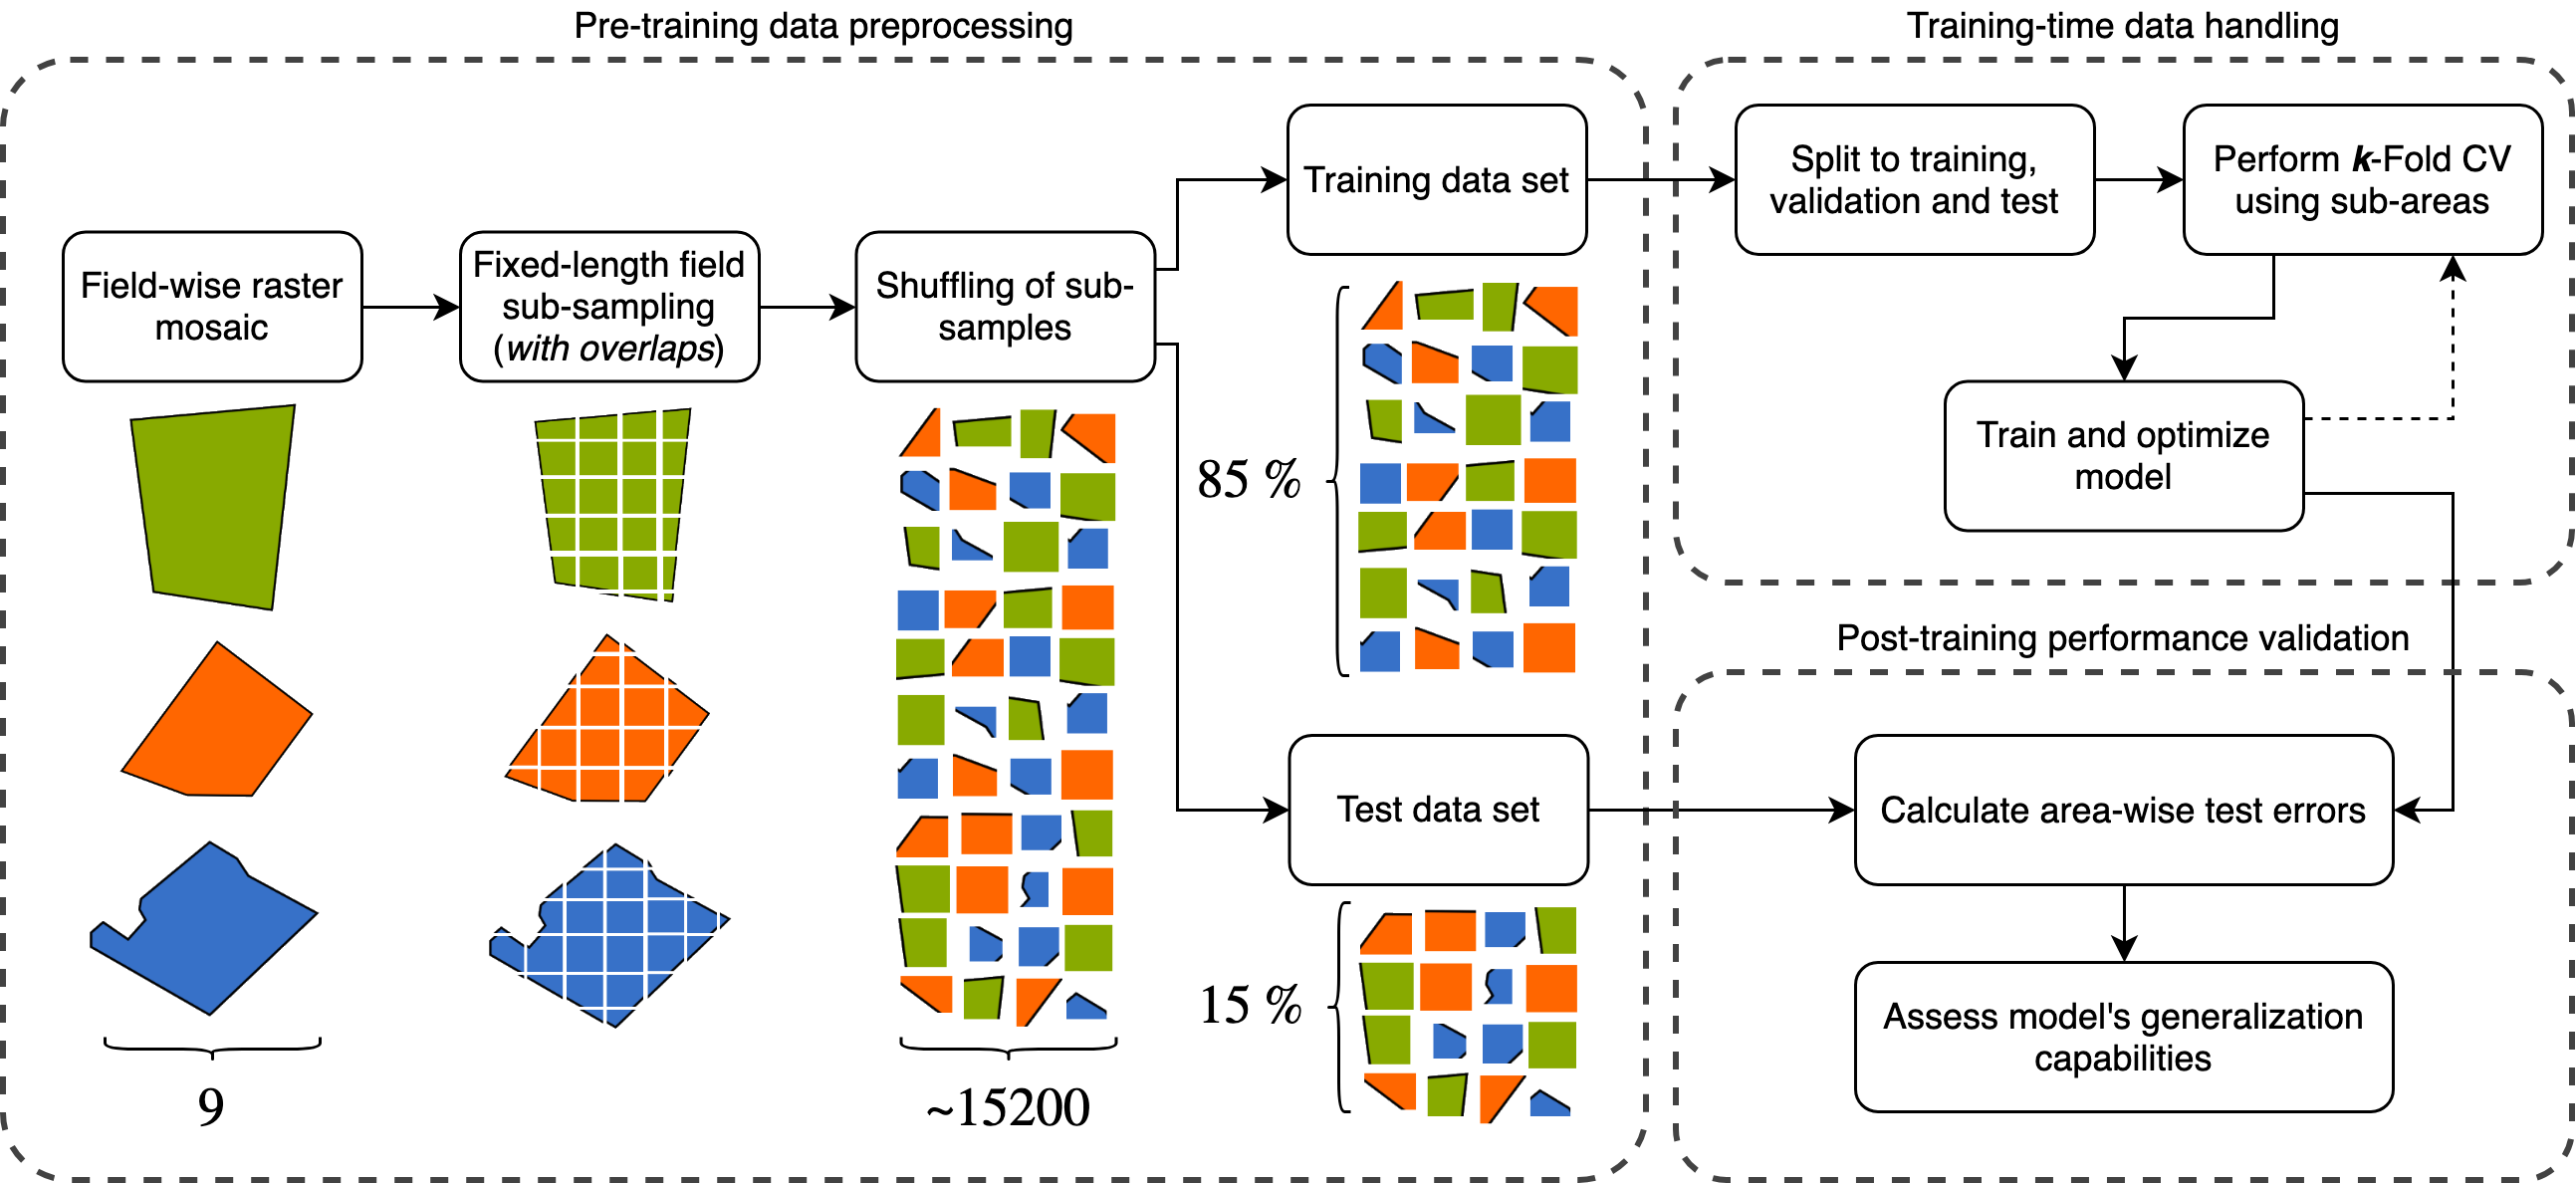
\includegraphics[width = \textwidth]{images/i-data-handling.png}
    \caption{The process of data preparation prior to and during training (reproduced from [I]).}
    \label{fig:i-data-handling}
\end{figure}

The basic architecture of the implemented CNN model follows closely the one reported in \cite{Krizhevsky2017a}. The general topology of the network is depicted in Figure \ref{fig:i-cnn}. The model was implemented using the PyTorch framework \cite{paszke2017automatic}. The model's inputs can be single-band or multi-band images ($B$) with varying dimensions ($D$). The network has at least two convolutional layers accompanied with two fully connected layers. The depth of the network is controlled by the number of intermediary convolutional layers. The last convolutional layer has 128 kernels while the intermediary layers have 64 kernels. Max pooling is applied only in the first and last convolutional layers so that the size of the data representation stays consistent when network depth is varied. The model uses non-overlapping pooling windows with pooling window size of 5 and a pooling stride matching the pooling window size. Pooling is applied only in the first and the last convolutional layers. Rectified linear units (ReLU) \cite{He2015} are used for layer-wise non-linear activation functions. This way our network is also scalable with respect to the number of layers. Two FC layers with 1024 neurons per layer are used to produce the final output from the CNN outputs.

\begin{figure}[ht]
\centering
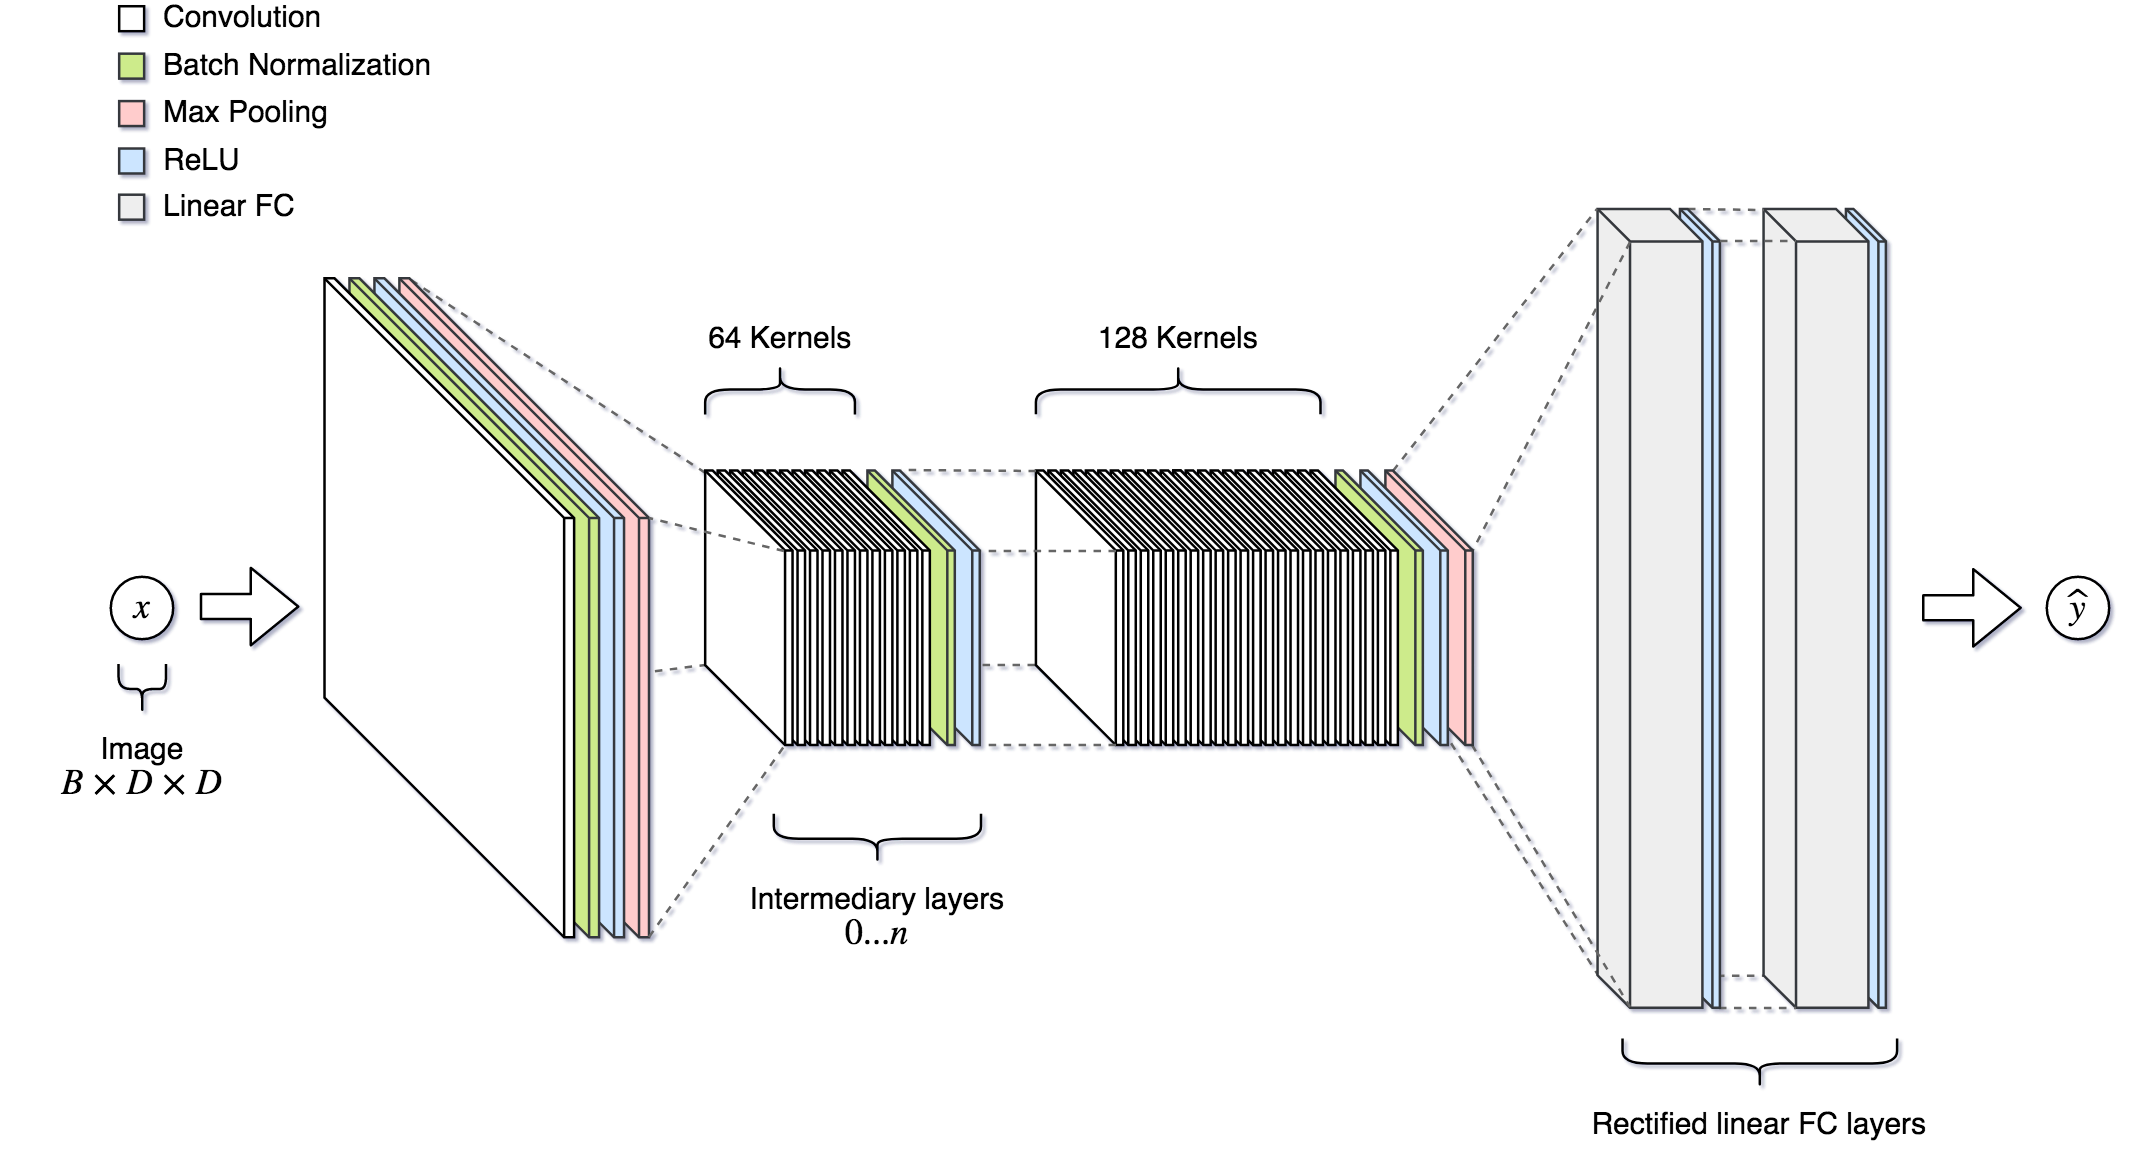
\includegraphics[width = \textwidth]{Images/i-cnn.png}
\caption{The overall topology of the implemented CNN (reproduced from [I]). }
\label{fig:i-cnn}
\end{figure}

Finding the optimal configuration of any deep learning network is an iterative process, where the model's parameters are initialized and tuned multiple times. The best training algorithm was evaluated among three options: Stochastic Gradient Descent with momentum (SGD-momentum) \cite{Bottou1998}, RMSprop \cite{Hinton2014} and Adadelta \cite{Zeiler2012} as suggested in \cite{Goodfellow-et-al-2016} and present in \cite{Karpathy2017}. Out of these, Adadelta performed the best. Optimizer parameters, such as learning rate, coefficient of using past gradients during backpropagation and weight decay, were tuned using random search \cite{Bergstra2012}. Other parameters were tuned by testing various values from predefined selections. These parameters were

\begin{itemize}
    \item input sample batch size (from $2^5$ to $2^{10}$)
    \item the number of intermediate convolutional layers (from 4 to 12)
    \item input data type (NDVI or RGB)
    \item frame side length (10m 20m or 40m)
    \item early stopping patience (from 10 to 50).
\end{itemize}

The lowest test set error of 484 kg/ha MAE and 8.8 \% MAPE was achieved using RGB data from the beginning of the growing season, i.e. pre-June images. R$^2$ score was 0.857. The best model consisted of six convolutional layers followed by two fully connected layers, using weight decay regularization with the coefficient being $10^{-3}$ and early stopping with patience of 50. The optimizer was also tuned, with the optimal values for learning rate and the coefficient adjusting the effect of past iterations' error corrections being $8 \times 10^{-3}$ and 0.58, respectively. The results show that the lowest test errors were achieved with the largest frame side length of 40 m. 

The best performing model was also utilized in a case study of six fields containing mostly barley, together accounting for 54.2 ha of land area and located near the city of Pori [II]. Imaging and yield acquisition methods were identical to [I], with some overlaps in the field-wise data. The crop yield prediction results indicate a consistent pattern of overestimating low yields and underestimating high yields. This is shown in Figure~\ref{fig:ii-FigurePallette}, where all values are absolute and in kg/ha. Over the six fields, the model attained 0.798 R$^2$, on average. Field-wise MAPE boxplots are depicted in Figure~\ref{fig:ii-boxplots}. 

\begin{figure}[htb]
    \centering
    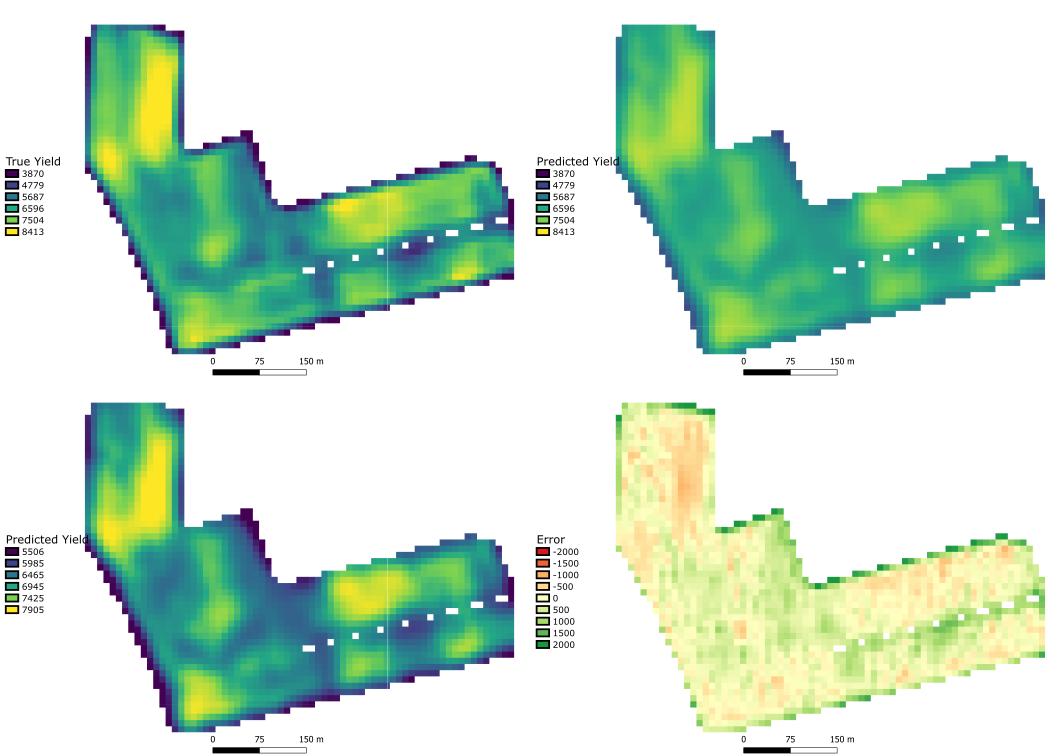
\includegraphics[width = \textwidth]{Images/ii-FigurePallette.png}
    \caption{Visualisation of the true and predicted yield of a field (reproduced from [II]). Images of true and predicted yields in the top row share a similar scale. Bottom left image is scaled to predicted values only. Bottom right image depicts the error between true and predicted yield. Units are in kg/ha.}
    \label{fig:ii-FigurePallette}
\end{figure}

\begin{figure}[htb]
    \centering
    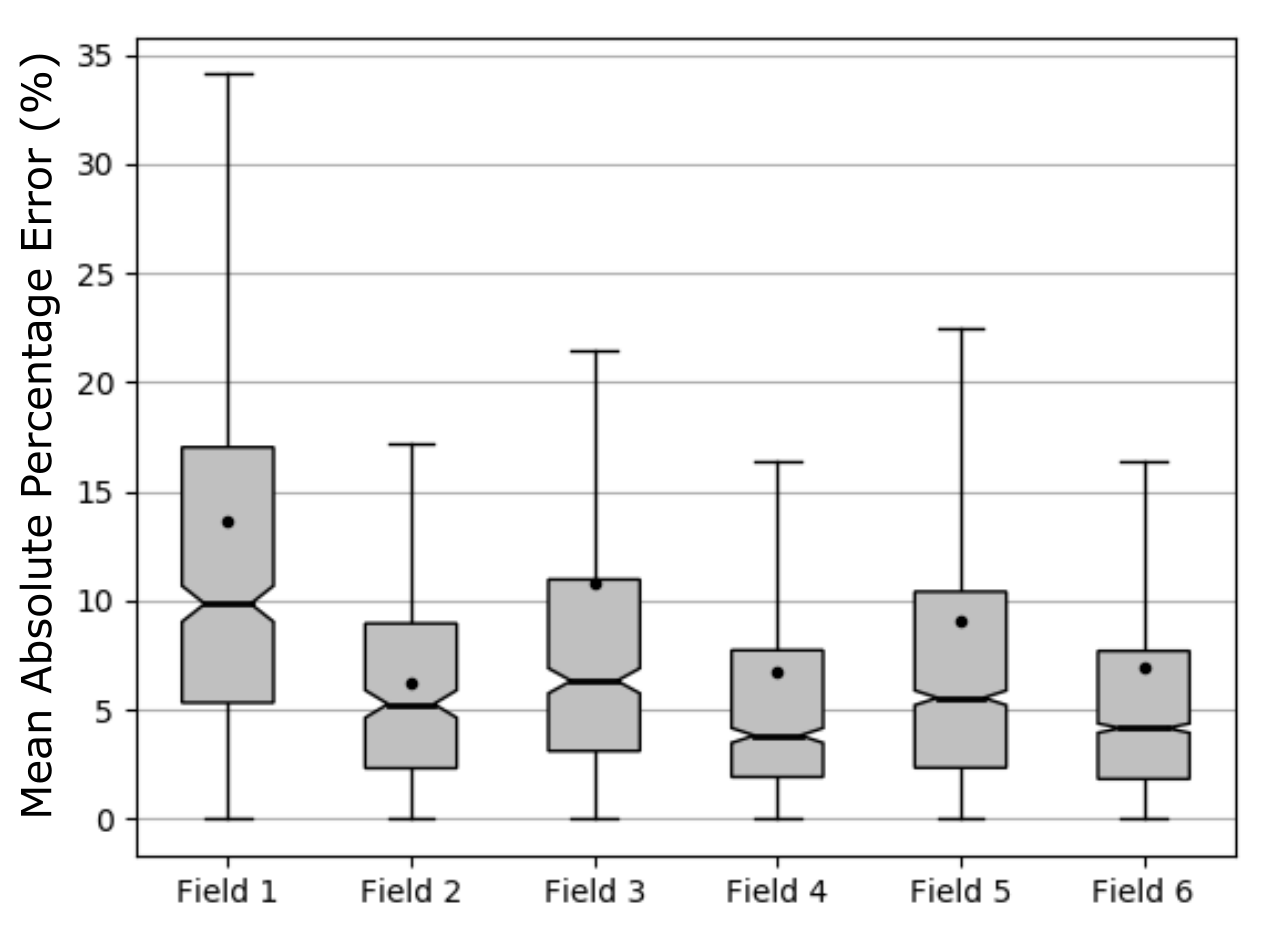
\includegraphics[width = 0.6\textwidth]{Images/ii-MAPE_boxplots.png}
    \caption{Boxplots of percentage error between true yield and predicted yield for each field (reproduced from [II]).}
    \label{fig:ii-boxplots}
\end{figure}

The model was also designed to be utilized as an AI engine in an Oskari-based (\emph{www.oskari.org}, MIT \& EUPL licensed) geospatial data mapping and farming decision support system. Through the web portal farmers can access their personal, authenticated accounts, upload data for visualization and call on AI based analytical tools for decision support.

\subsection{Sequence of inputs to single target}
\label{subsec:sequence-input-results}

In [IV] we examined the effect of time, as an additional feature, on intra-field yield prediction. Especially, capabilities of deep learning time series models utilizing UAV remote sensing time series data as their inputs were focused on. The objectives were two-fold: to see if the performance of the point-in-time model of [I] could be surpassed using spatiotemporal deep learning model architectures and to see which spatiotemporal architecture would perform better in the same task. The usability of spatiotemporal models was evaluated in two settings, end-of-season (full sequence) and in-season (limited sequence) prediction. Three model architectures were designed, trained and evaluated: a CNN-LSTM \cite{Sainath2015}, a convolutional LSTM \cite{Shi2015a} and a 3D-CNN \cite{Tran2015}. These models utilize the properties of CNNs and LSTM networks them to perform spatiotemporal modelling. The main contribution of the study was to perform time series based intra-field yield prediction with multi-temporal data collected during the growing season with UAVs.

Nine crop fields totaling to approximately 85 ha and having wheat, barley and oats as the crop varieties, were included in the study. The field-wise data was acquired during year 2018 in the proximity of Pori, Finland (61$^\circ$29'6.5''N, 21$^\circ$47'50.7''E). Specific information about the fields is given in Table~\ref{tab:iv-field-info}. The acquisition of input and target data was similar to [I]. 

\begin{table}[ht]
    \scriptsize
    \centering
    \caption{The fields selected for the multitemporal study in the proximity of Pori, Finland (reproduced from [IV]).}
    \label{tab:iv-field-info}
    \vspace{0.3cm}
    \begin{tabular}{@{}cccccc@{}}
    \toprule
    \textbf{\makecell{Field\\\#}} & \textbf{\makecell{Size \\ (ha)}} & \textbf{\makecell{Mean yield \\ (kg/ha)}} & \textbf{\makecell{Crop\\(\textit{Variety})}} & \textbf{\makecell{Thermal\\time}} & \textbf{\makecell{Sowing\\date}} \\ \midrule
    1                             & 11.11                            & 4349.1                                    & \makecell{Wheat\\(\textit{Mistral})}         & 1290.3                            & 13 May                           \\
    2                             & 7.59                             & 5157.6                                    & \makecell{Wheat\\(\textit{Mistral})}         & 1316.8                            & 14 May                           \\
    3                             & 11.77                            & 5534.3                                    & \makecell{Barley\\(\textit{Zebra})}          & 1179.9                            & 12 May                           \\
    4                             & 11.08                            & 3727.5                                    & \makecell{Barley\\(\textit{Zebra})}          & 1181.3                            & 11 May                           \\
    5                             & 7.88                             & 4166.9                                    & \makecell{Barley\\(\textit{RGT Planet})}     & 1127.6                            & 16 May                           \\
    6                             & 13.05                            & 4227.9                                    & \makecell{Barley\\(\textit{RGT Planet})}     & 1117.1                            & 19 May                           \\
    7                             & 7.61                             & 6668.5                                    & \makecell{Oats\\(\textit{Ringsaker})}        & 1223.4                            & 17 May                           \\
    8                             & 7.77                             & 5788.2                                    & \makecell{Barley\\(\textit{Harbringer})}     & 1136.1                            & 21 May                           \\
    9                             & 7.24                             & 6166.0                                    & \makecell{Oats\\(\textit{Ringsaker})}        & 1216.4                            & 18 May                           \\ \bottomrule
    \end{tabular}
\end{table}

Images of the fields were acquired with a SEQUIOA (Parrot Drone SAS, Paris, France) multispectral camera mounted on a Airinov Solo 3DR (Parrot Drone SAS, Paris, France) UAV on a weekly basis for 15 consecutive weeks. To encode passing of time for the temporal models, weather data was acquired from the open interface provided by the Finnish Meteorological Institute for Pori area. Being a common way to express crop growth phase, the cumulative temperature was utilized as the temporal feature in the input data. Temporally varying but spatially constant cumulative temperature was added as an additional layer in conjunction with the RGB layers to have the data contain necessary information for temporal feature learning. The targets data, crop yields, were acquired during the harvest of each field. The harvesters were equipped with either a Trimble Navigation (Sunnyvale, California, USA) CFX 750 or John Deere (Moline, Illinois, USA) Greenstar 1 yield mapping sensor systems, which produce a cloud of geolocated points with multivariate information about the harvest for each point in vector format.

The fields were split into smaller overlapping frames of size 40 $\times$ 40 m with a lateral and vertical step of 10 m. Sequences of frames of fixed width and height were extracted from sequences of field plot images and corresponding weather data as the input data. The input frames were then geolocationally paired with corresponding yield data to form input-target pairs. A total of 2586 sequences, 15 geolocationally matching frame rasters per sequence, were extracted from the data. Lastly, data was shuffled and split to training and test sets with a 70\%/30\% ratio, respectively. The general process of generating the frames is depicted in Figure~\ref{fig:iv-data-processing}.

\begin{figure}[htb]
    \centering
    \includegraphics[width = 0.8\textwidth]{images/iv-data-processing.png}
    \caption{Input frame sequence and target average yield extraction process (reproduced from [IV]).} 
    \label{fig:iv-data-processing}
\end{figure}

All models we trained with random search \cite{Bergstra2012}. For the CNN-LSTM, the CNN of the model was first trained separately with distinct frames, i.e. point-in-time data. Training the model from scratch was required due to changes in input channel count. It was trained according to the best results of [I], using Adadelta \cite{Zeiler2012} as the optimizer. For the spatiotemporal models, Adam \cite{Kingma2015} was used as the optimizing algorithm for each model architecture akin to \cite{Rustowicz2019}, \cite{Yaramasu2020} and \cite{Liu2017}. The spatiotemporal models were trained with frame sequences. A total of 950 models were trained, with 300 for each spatiotemporal model and 50 for the CNN of the CNN-LSTM. 

In the first phase the models were trained to perform end-of-season predictions with full length frame sequences. The trained models were evaluated with a hold-out test set and the results are given in Table~\ref{tab:iv-test-results}. The number of trainable parameters indicate the model complexity and the best values are in bold. Best performance was achieved with the 3D-CNN architecture. 
 
% Please add the following required packages to your document preamble:
% \usepackage{booktabs}
\begin{table}[htb]
    \scriptsize
    \centering
    \caption{The end-of-season prediction performance metrics of the best spatiotemporal models (reproduced from [IV]).}
    \label{tab:iv-test-results}
    \vspace{0.3cm}
    \begin{tabular}{@{}llllll@{}}
    \toprule
    \textbf{Model} & \textbf{\begin{tabular}[c]{@{}l@{}}Test RMSE\\(kg/ha)\end{tabular}} & \textbf{\begin{tabular}[c]{@{}l@{}}Test MAE\\(kg/ha)\end{tabular}} & \textbf{\begin{tabular}[c]{@{}l@{}}Test MAPE\\(\%)\end{tabular}} & \textbf{\begin{tabular}[c]{@{}l@{}}Test R$^2$\\ -\end{tabular}} & \textbf{\begin{tabular}[c]{@{}l@{}}Trainable\\ parameters\end{tabular}} \\ \midrule
    Pretrained CNN & 692.8                                                               & 472.7                                                              & 10.95                                                            & 0.780                                                           & 2.72$\times 10^{6}$                                                     \\
    CNN-LSTM       & 456.1                                                               & 329.5                                                              & 7.97                                                             & 0.905                                                           & 2.94$\times 10^{6}$                                                     \\
    ConvLSTM       & 1190.3                                                              & 926.9                                                              & 22.47                                                            & 0.349                                                           & 9.03$\times 10^{5}$                                                     \\
    3D-CNN         & \textbf{289.5}                                                      & \textbf{219.9}                                                     & \textbf{5.51}                                                    & \textbf{0.962}                                                  & 7.48$\times 10^{6}$                                                     \\ \bottomrule
    \end{tabular}
\end{table}

In-season prediction performance was evaluated with the best performing 3D-CNN model configuration and using data from an actionable time frame from the beginning of the growing season. Multiple input data configuration were tested, forming varying sequences of 3 to 5 frames from five first weeks of imaging (weeks 21 to 25 of 2018). Overall, the best perfoming in-season sequence cconfiguration in terms of MAE was the four-week-long sequence taken from the beginning of the season (weeks 21 to 24) with 292.8 kg/ha MAE, 7.17 \% MAPE and 0.929 R$^2$. Visualized prediction results are illustrated in Figure~\ref{fig:iv-true-pred} with a 10 meter step between predicted points. 

\begin{figure}[htb]
    \centering
    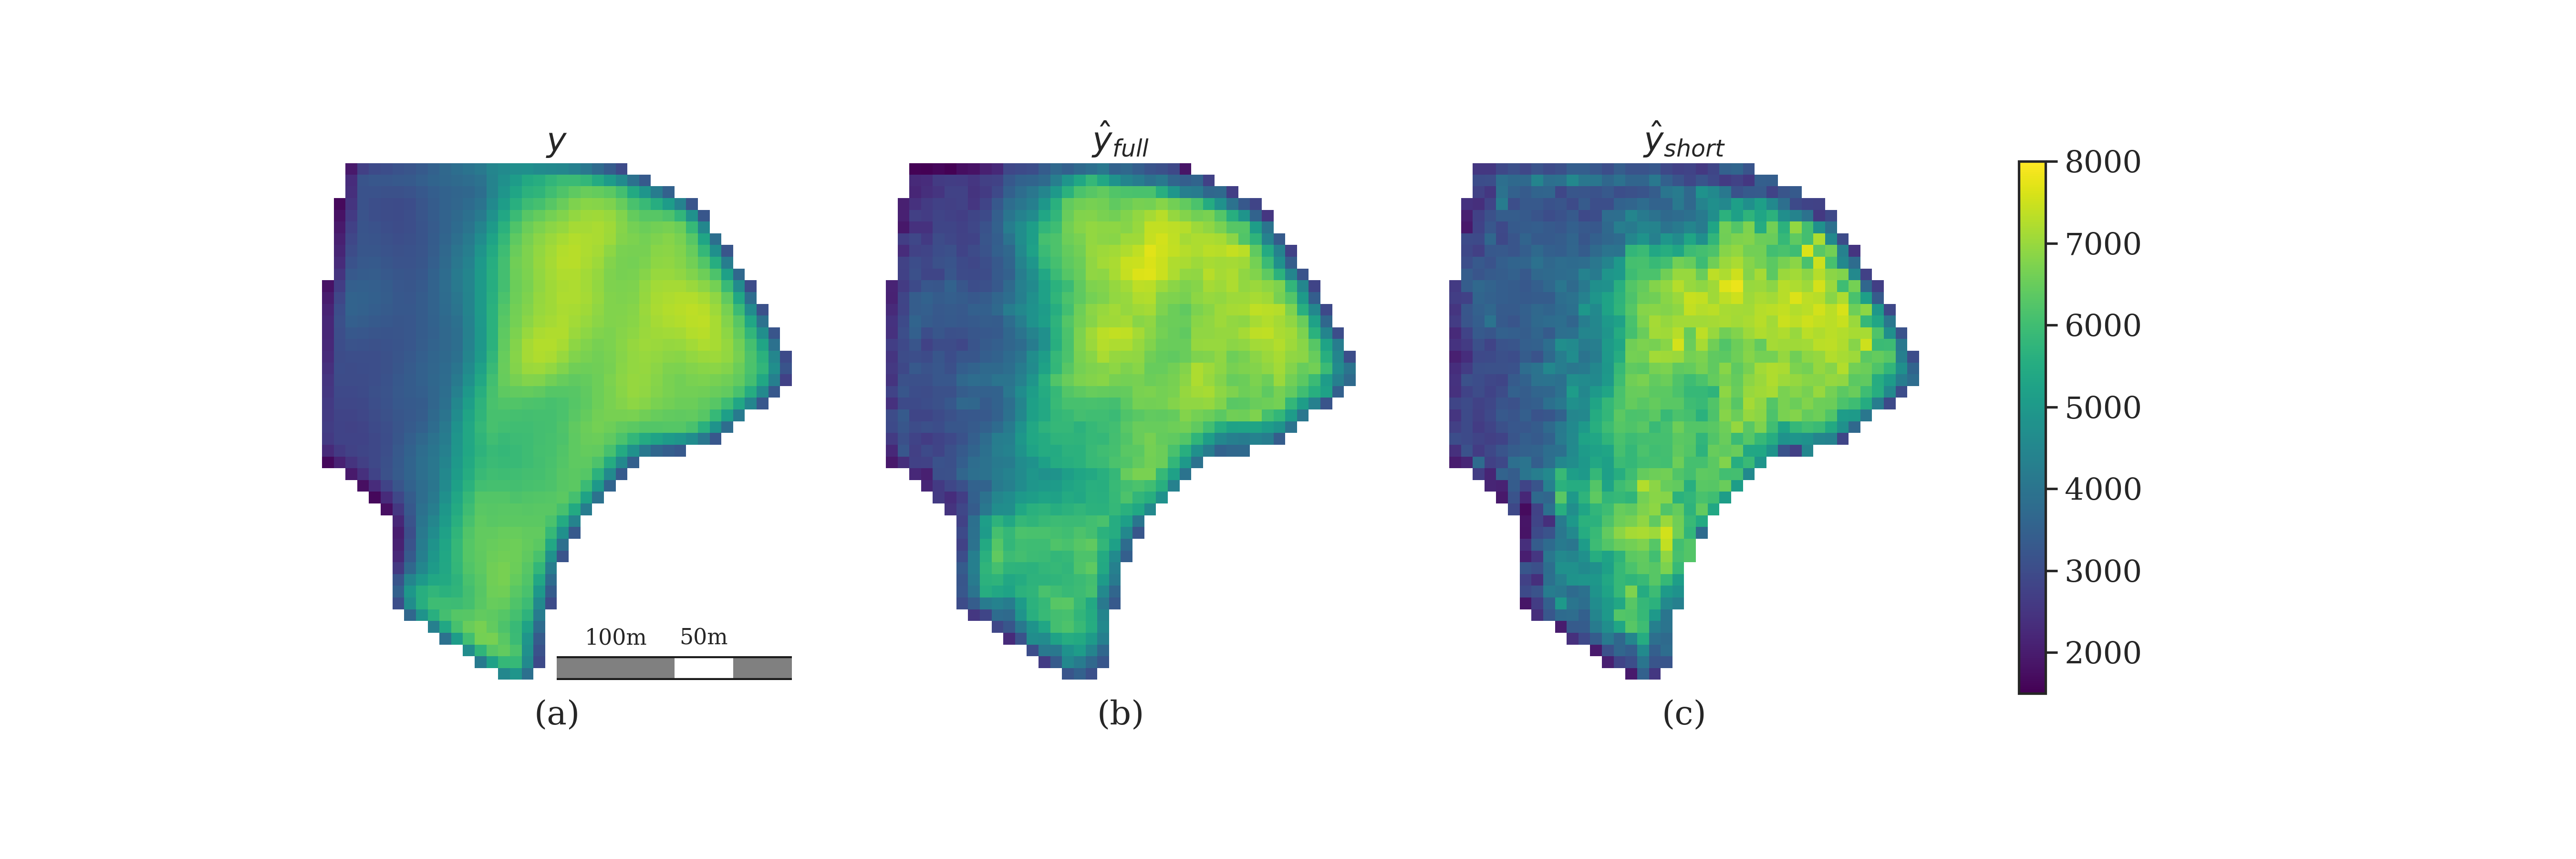
\includegraphics[width = \textwidth]{Images/iv-true_pred.png}
    \caption{Frame-based 3D-CNN model performances against true yield data (reproduced from [IV]).}
    \label{fig:iv-true-pred}
\end{figure}

\section{Remote sensing data evaluation}
\label{sec:input-assessment-results}


\subsection{Additional input sources}
\label{subsec:additional-inputs-results}

In [V] the effects of additional field-related spatial or spatial-like data on the intra-field crop yield prediction capabilities were studied. The model architecture was taken from [I] and a baseline was trained with RGB data from the earlier half of the growing season of 2018 (weeks 21 to 26). The objective of the study was to assess crop yield prediction capabilities with the best CNN model composition from [I] by varying the input data configurations with additional data. Additional data sources included data from the following sources: local weather stations, soil samplings, soil sensors and Sentinel-2 satellite system. Disregarding the changing number of input channels, the architectural and optimizer related hyperparameters were not changed to better isolate the effects of different input configurations on the yield estimation performance.

Four crop fields were selected for data acquisition in the vicinity of Pori, Finland (61$^\circ$29'6.5''N, 21$^\circ$47'50.7''E) for the growing season of 2018. The field information is provided in Table~\ref{tab:v-field-info}. The multisource input data for the fields consists of UAV-based RGB images, multispectral Sentinel-2 \cite{ESAS2} satellite data, sparsely collected and analyzed soil samplings, machine-collected soil information, topography information and local weather station data. 

\begin{table}[htb]
    \scriptsize
    \centering
    \caption{The fields selected for multisource study in the proximity of Pori, Finland (reproduced from [V]).}
    \label{tab:v-field-info}
    \vspace{0.3cm}
    \begin{tabular}{@{}cccccc@{}}
    \toprule
    \textbf{\makecell{Field\\\#}} & \textbf{\makecell{Size \\ (ha)}} & \textbf{\makecell{Mean yield \\ (kg/ha)}} & \textbf{\makecell{Crop\\(\textit{Variety})}} & \textbf{\makecell{Thermal\\time ($^{\circ}$C)}} & \textbf{\makecell{Sowing\\date}} \\ \midrule
    1                             & 7.59                             & 5157.6                                    & \makecell{Wheat\\(\textit{Mistral})}         & 1316.8                            & 14 May                           \\
    2                             & 11.77                            & 5534.3                                    & \makecell{Barley\\(\textit{Zebra})}          & 1179.9                            & 12 May                           \\
    3                             & 7.88                             & 4166.9                                    & \makecell{Barley\\(\textit{RGT Planet})}     & 1127.6                            & 16 May                           \\
    4                             & 7.24                             & 6166.0                                    & \makecell{Oats\\(\textit{Ringsaker})}        & 1216.4                            & 18 May                           \\ \bottomrule
    \end{tabular}
\end{table}

General information about the original data sources are given in Table~\ref{tab:v-data-general}. UAV data was acquired with weekly overfligths of each field using a SEQUIOA (Parrot Drone SAS, Paris, France) multispectral camera mounted on a Airinov Solo 3DR (Parrot Drone SAS, Paris, France) UAV. The Sentinel-2 satellite data for the fields was acquired from the Copernicus Open Access Hub (European Space Agency, Paris, France), date-matched with UAV-images. Soil samples were collected manually during November 2018 from the fields with 50 m steps by ProAgria, an agronomic counseling instution, and sent to a Eurofins (Eurofins Viljavuuspalvelu, Mikkeli, Finland) laboratory for further analysis. An MSP3 soil scanner (Veris Technologies, Salina, Kansas, USA) was used to map the fields at depths of 0-30 cm and 30-90 cm. The measurements were performed during April and May of 2019. Lidar-based topographical information was acquired from the open-access data portal of the National Land Survey of Finland. Weather data was collected with two separately located Vantage Pro2 (Davis Instruments, Hayward, California, USA) weather stations. Yield data was acquired during the harvest of 2018 with yield mapping sensor devices attached to the harvesters, either with a CFX 750 (Trimble Navigation, Sunnyvale, California, USA) or Greenstar 1 (John Deere, Molinde, Illinois, USA). 

% Please add the following required packages to your document preamble:
% \usepackage{booktabs}
\begin{table}[htb]
    \centering
    \scriptsize
    \caption{General information of data sources and their original formats (reproduced from [V]).}
    \label{tab:v-data-general}
    \begin{tabular}{@{}lllll@{}}
    \toprule
    \textbf{Source} & \textbf{Type} & \textbf{Resolution/Step} & \textbf{Multitemporal} & \textbf{Channels} \\ \midrule
    UAV             & Raster        & 0.3125 m/px              & Yes                    & 3                 \\
    Sentinel-2     & Raster        & {[}10,20,60{]} m/px      & Yes                    & 19                \\
    Soil samples    & Vector        & 50 m                     & No                     & 8                 \\
    Veris MSP3      & Vector        & 20 m                     & No                     & 6                 \\
    Topography      & Vector        & 2 m                      & No                     & 1                 \\
    Weather         & Tabular       & -                        & Yes                    & 2                 \\
    Yield           & Vector        & Varying                  & No                     & 1                 \\ \bottomrule
    \end{tabular}
\end{table}

All inputs were harmonized to the spatial resolution of the RGB data, 0.3125~m/px by interpolating coarser data sources with GDAL utility's \texttt{gdal\_grid} program with \texttt{invdist:power=3:smoothing=20} interpolation algorithm. After that, overlapping frames were extracted from the data for each week, resulting in a total of 16375 frames. As the number of unique fields was low, maximizing the sample variability the model sees during training was necessary. The data was divided to distinct training, validation and test sets according to the UAV image acquisition week and shuffled to eliminate spatial autocorrelation in subsequent samples due to overlapping frame extraction. 

The last step of data processing was to build the data sets for different data source configurations. Four distinct configurations were considered:

\begin{itemize}
    \item \emph{RGB Only}, which uses UAV RGB data only
    \item \emph{No S2}, which uses UAV, soil, Veris MSP3, topography and weather data
    \item \emph{S2 Raw}, which adds Sentinel-2 raw wavelength band data to \emph{No S2}
    \item \emph{S2 Full}, which adds calculated Sentinel-2 Level-2A product layers to \emph{S2 Raw}.
\end{itemize}

Ten models were trained for each configuration to account for random initialization of the models inner parameters (weights) and the best models for each configuration were considered. The performance with larger number of fields using UAV RGB data has already been extensively studied in [I] and [IV]. Thus, training a model with only UAV RGB data provides a studied baseline to which models trained with additional data can be compared. The baseline model using UAV RGB data only attained 1055.7 kg/ha test RMSE, 18.2\% test MAPE and 0.343 test R$^2$. The best performing data configuration was \emph{S2 Full} with 364.1 kg/ha test RMSE, 5.18\% test MAPE and 0.922 test R$^2$ using all 39 layers of input data for each extracted frame. Compared to the baseline \emph{RGB Only} model, the \emph{S2 Full} attained 65.6\% lower RMSE, 67.3\% lower MAE, 71.5\% better MAPE and 0.579 higher R$^2$ with the test set. Generally every model with multisource inputs performed better than the baseline model. This is shown in Table~\ref{tab:v-relative-results}.

% Please add the following required packages to your document preamble:
% \usepackage{booktabs}
% \usepackage{multirow}
\begin{table}[htb]
    \scriptsize
    \centering
    \caption{The relative performance of the models trained with distinct multisource input data configurations to the baseline \emph{RGB Only} model (reproduced from [V]).}
    \label{tab:v-relative-results}
    \begin{tabular}{@{}lllll@{}}
    \toprule
    \multirow{2}{*}{\textbf{\begin{tabular}[c]{@{}l@{}}Data\\ Setting\end{tabular}}} & \multicolumn{4}{c}{\textbf{Relative change from \emph{RGB Only}}}                                                                                                                                                                                                                         \\
                                                                                     & \textbf{Test RMSE} & \textbf{Test MAE} & \textbf{Test MAPE} & \textbf{Test R$^2$} \\ \midrule
    No S2                                                                            & -15.5\%            & -17.2\%           & -18.7\%            & +0.188               \\
    S2 Raw                                                                           & -56.3\%            & -59.4\%           & -61.9\%            & +0.532               \\
    S2 Full                                                                          & \textbf{-65.6\%}   & \textbf{-67.3\%}  & \textbf{-71.5\%}   & \textbf{+0.579}      \\ \bottomrule
    \end{tabular}
\end{table}


\subsection{Satellite data reliability}
\label{subsec:satellite-quality-results}

Data from the Sentinel-2 satellites are intensively used for various applications such as land use and vegetation mapping or crop monitoring. Depending on climate conditions in the region of interest, one of the main obstacles in using the data for practical monitoring purposes is cloud coverage. Currently, the cloud mask of the Sentinel data is available in the form of the Level 1C product containing vector layers of dense and cirrus clouds. Also, the percentage of cloudy pixels (dense and cirrus) in the mask are provided. The Level 2A product further processes the Level 1C data to obtain the Scene Classification layer with cloud and cirrus probability values at 60 m spatial resolution. According to Coluzzi et.al. \cite{Coluzzi2018}, caution has to be taken when using the provided cloud masks and improved cloud detection algorithms are welcome.

Therefore, a random forest classifier was trained to assess cloud cover in Sentinel-2 data in [III], using data acquired from crop fields by UAVs as ground truth for cloudless data. For cloudless multispectral ground truth data, ten crop fields were selected for imaging during 2018 and 2019 in the vicinity of Pori, Finland (61$^\circ$29'N, 21$^\circ$48'E). The fields were imaged approximately weekly with two distinct drones both years, using 3DR Solo (Parrot Drone SAS, Paris, France) for the year 2018 and Disco-Pro AG (Parrot Drone SAS, Paris, France) for 2019. The drones were equipped with similar SEQUIOA (Parrot Drone SAS, Paris, France) multispectral cameras. Half of the fields had wheat (\textit{Zebra/Mistral}), three had barley (\textit{Harbringer/RGT Planet}) and two remaining had oats (\textit{Ringsaker}) as the cultivated crop. The total area of the selected fields was approximately 93 ha. The drone images were downsampled to match the highest resolution available in Sentinel-2 images, 10 m/px. In total, 288 images of distinct crop field images constituted the complete data set.

However, comparing absolute values across bands for two different sensors and imaging platforms proved out to be difficult, as the data would require scaling to an unkown global maximum for Sentinel-2. Thus, using the NDVI values calculated from both data sources (UAV and Sentinel-2) was deemed appropriate due to the index providing normalized and thus comparable data between distinct imaging systems.

To facilitate data based modelling in a supervised setting, target values are required. Due to UAV flight altitude of 150 m eters, Sentinel-2 data can be seen as being cloudless when the NDVI values for a field are similar to the UAV based values as possible. Thus, the task of classification is that of classifying Sentinel-2 data either similar or dissimilar to the UAV data. The similarity for a single pixel-corresponding area is determined by

\begin{equation}
    sim_{(s,d)} = \begin{cases}  1, & |s-d| \leq threshold \\ 
    0, & \mbox{otherwise} 
    \end{cases}
    \label{eq:iii-similarity}
\end{equation}

\noindent where $s$ and $d$ are spatially and temporally aligned NDVI pixels for a field from the satellite and drone sources respectively. Similarity indicates that Sentinel-2 data is cloudless, while dissimilarity indicates cloudiness. The threshold had to be determined via empirical analysis. The task of determining the threshold for labeling is a task of balancing between (1) capturing as much similarities while (2) still excluding as many dissimilarities as possible. Using Students $t$-test, a total of 15 statistically similar ($p = 0.01$) week-aligned NVDI image pairs were found. Usign similar images, the threshold of similarity was empirically determined by comparing the ratio of pixels deemed similar produced by various thresholds with Equation~\ref{eq:iii-similarity}. The threshold of 0.075 absolute difference in NDVI was selected. A single image pair with the calculated similarity map is shown in Fig.~\ref{fig:iii-s2-drone-comparison}. The first two figures depict the NDVI maps from corresponding sources. The third figure shows the absolute difference between the aligned Sentinel-2 and drone NDVI values. The fourth figure shows the thresholded absolute difference, indicating areas where the NDVI images are similar enough. 

\begin{figure*}[htb]
    \centering
    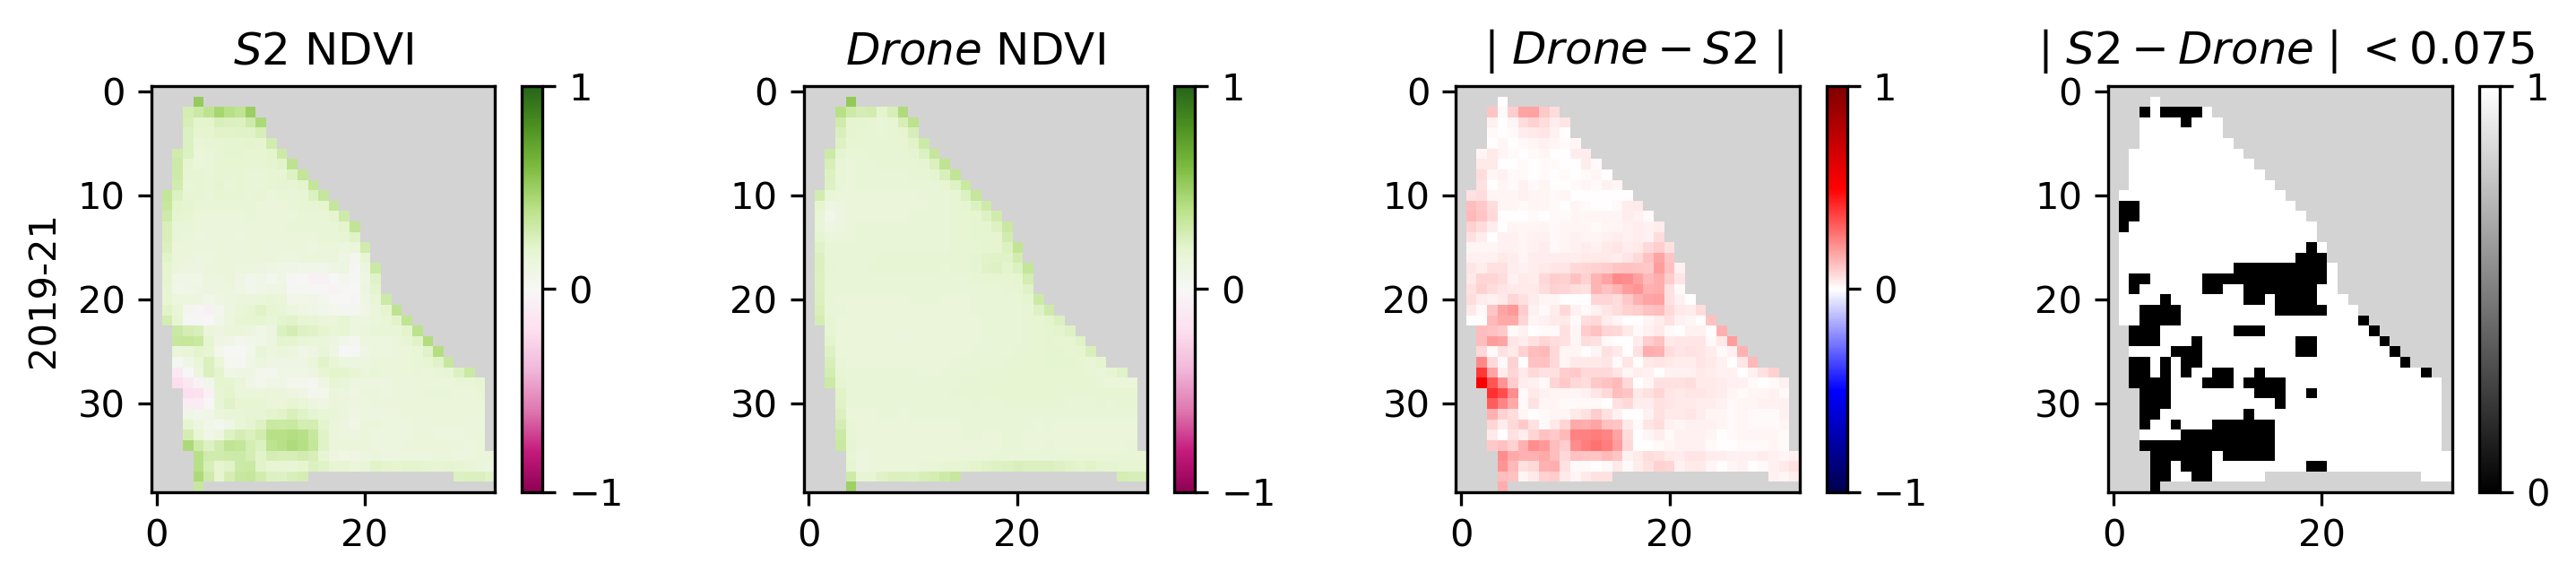
\includegraphics[width=\textwidth]{./Images/iii-targets-8860198450-2019-21.png}
    \caption{A visualization of a single week-aligned Sentinel-2 and drone NDVI image pair with the absolute difference and the similarity map (reproduced from [III]).}
    \label{fig:iii-s2-drone-comparison}
\end{figure*}

\begin{table}[htb]
    \centering
    \scriptsize
    \caption{The confusion matrix of similarity label predictions (reproduced from [III]).}
    \label{tab:iii-confusion-matrix}
    \begin{tabular}{@{}ccc@{}}
    \toprule
    Pred/True  & \textbf{0}                                                              & \textbf{1}                                         \\ \midrule
    \textbf{0} & \multicolumn{1}{c|}{\begin{tabular}[c]{@{}c@{}}TP\\ 23237\end{tabular}} & \begin{tabular}[c]{@{}c@{}}FP\\ 2580\end{tabular}  \\ \cmidrule(l){2-3} 
    \textbf{1} & \multicolumn{1}{c|}{\begin{tabular}[c]{@{}c@{}}FN\\ 1807\end{tabular}}  & \begin{tabular}[c]{@{}c@{}}TN\\ 36037\end{tabular} \\ \bottomrule
    \end{tabular}
\end{table}

\begin{table}[htb]
    \centering
    \scriptsize
    \caption{Similarity estimates with hold out test data (reproduced from [III]).}
    \label{tab:iii-model-s2-comparison}
    \begin{tabular}{@{}lllllll@{}}
    \toprule
                                 & \multicolumn{3}{c}{$y = 0$}                         & \multicolumn{3}{c}{$y = 1$}     \\
                                 & Mean          & Std   & Median                   & Mean          & Std  & Median \\ \midrule
    Model                        & \textbf{0.07} & 0.25 & \multicolumn{1}{l|}{0.00} & 0.93          & 0.26 & 1.00  \\
    $\text{CLDPRB}_{\text{SIM}}$ & 0.45          & 0.45 & \multicolumn{1}{l|}{0.26} & \textbf{0.97} & 0.14 & 1.00  \\
    $\text{SCL}_{\text{SIM}}$    & 0.28          & 0.45 & \multicolumn{1}{l|}{0.00} & 0.95          & 0.22 & 1.00  \\ \midrule
    Samples                      & \multicolumn{3}{c}{38617}                           & \multicolumn{3}{c}{25044}       \\ \bottomrule
    \end{tabular}
\end{table}

The thresholded binary value maps constitute the target data for pixel-wise binary classification, while Sentinel-2 data was used as inputs. A total of 381972 input-target samples (pixels) were extracted from the source data. The samples were then shuffled and split into training and test data sets with 190986 and 63661 samples, correspondingly. Due to using data in tabular manner, where an input pixel contains several values and spatial dependencies are not modelled, a decision tree based random forest was deemed an appropriate model to use. The confusion matrix of model predictions against true labels with test data is shown in Table~\ref{tab:iii-confusion-matrix}.

The comparison of sample-wise similarity estimations between the trained model and Sentinel-2 data products are given in Table~\ref{tab:iii-model-s2-comparison}. The estimates are given both for when the true target value was 0 (satellite differed from drone) and when it was 1 (satellite similar to drone). For cloudless Sentinel-2 data, the model performed close to existing cloudiness estimates provided with the data products. For cloudy data, the model performed significantly better.



\chapter{Conclusions and discussion}
\label{ch:conclusions}
Information relevant for decision making in agriculture can be extracted from heterogeneous remote sensing, environmental and intervention-derived data by means of machine learning. With advancements in computational technologies, the development and training of non-linear multilayer algorithms has become feasible. These methods are commonly referred to as deep learning. Probably the most widely used deep learning structure is that of CNNs, proved to be superior in a variety of image analysis tasks. Other common structure is the RNN network, which is used for modelling sequences of data. A common property of the deep learning structures is that training of the models is performed based on data, i.e., no predefined and pre-calculated feature vector is needed. This, however, implies that extensive data sets are required for training the models and the operation principles of the models are usually not revealed. Figure~\ref{fig:ii-AgroAI_Topics} depicts some application areas of deep learning in agriculture.

\begin{figure}[htb]
    \centering
    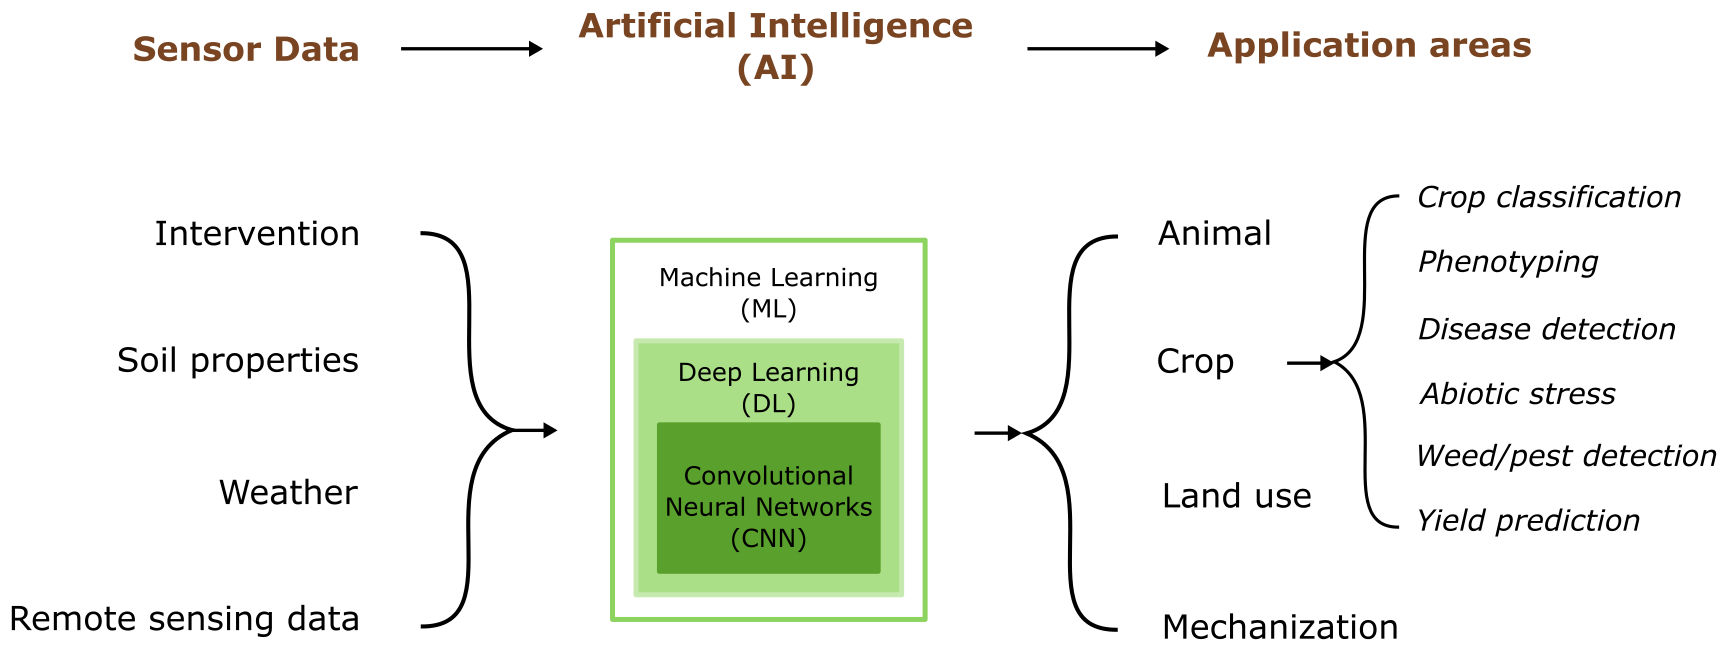
\includegraphics[width = 0.8\textwidth]{images/ii-AgroAI_Topics.png}
    \caption{Application areas of DL in agriculture.}
    \label{fig:ii-AgroAI_Topics}
\end{figure}

Remote sensing data can be acquired from satellites such as ESA’s Sentinel-2, for example. The problem with the satellite data is that if there is a cloud cover during the overflight of the satellite, no useful data are obtained. The spatial resolution of Sentinel-2 imagery is at best 10 m, which is enough for many applications but too low to allow using texture-based information in the images. Using UAVs for data acquisition offers better spatial resolution, the data acquisition time can be selected by the user and the data can be acquired also in cloudy conditions. Spectral wavelengths can be selected by using appropriate camera; UAV-mountable RGB-NIR cameras are available at affordable price. The drawback is that the UAV has to be operated locally and managing the data and extracting relevant information requires highly specialized skills.


\section{Deep learning and intra-field yield prediction}

The studies described in the publications [I], [II] and [IV] seek to predict yield at the intra-field scale using UAV based images in order to estimate yield variance within the field. This is in contrast to studies utilizing satellite-based, medium to low resolution data and predicting for considerably larger areas at lower spatial resolution. Models at intra-field scale offer the individual farmer the possibility of in-season monitoring of crop, which enables decision support systems for interventions necessary to achieve higher yields. 

Publication [I] is an important first step towards establishing a combined model for wheat and barley yield prediction in the Finnish continental subarctic climate. The long summer growing days in this region present a unique profile of temperature and photoperiod, justifying a region-specific deep learning model for these crops. By collecting high-resolution, namely 0.31 $\times$ 0.31 m/px, data using commercial off-the-shelf UAV and camera packages, the attention was focused on a spatial scale that enables us to predict intra-field yield variation within the context of individual farm crop monitoring. Considering that [I] models the yield based only on images, the resulting prediction error of 484 kg/ha test MAE, 8.8 \% test MAPE and 0.857 $R^2$-score is promising. The results of [I] indicate that the CNN models are capable of reasonable accurate yield estimates based on RGB images. This suggests that multiple spectral bands increase the information content in comparison to the condensed NDVI raster. From the results of [V] it can be suggested that complementing the RGB data with NIR channel might further enhance the prediction capabilities of the CNN model. Additionally, NIR-based vegetation indices could have improved modelling performance even more as discussed in \cite{Zhao2020}. Intra-field crop yield prediction based on multispectral UAV data based is, thus, a subject for a future study.

As further examined in [II], the case study with the CNN from [I] revealed some limitations of the model in yield prediction. The model underestimated/overestimated the yield in the regions of high/low yield values, respectively. Another limitation is related to yield data pre-processing. In some cases the polygons of yield data overlap causing errors in yield density maps.
 
In [IV] the feasibility of using spatiotemporal deep learning architectures in modelling crop yield at the intra-field scale was evaluated using high-resolution UAV data. With full sequence modelling, a 3D-CNN based architecture performed the best with 218.9 kg/ha test MAE, 5.51\% test MAPE and 0.962 test R$^2$-score. Compared to [I] using just a point-in-time single frame predictor with 484.3 kg/ha MAE and 8.8\% MAPE, the modelling performance was improved by 265.4 kg/ha MAE (54.8\% improvement) and 3.29\% MAPE (37.4\% improvement) with time series inputs. With a shorter sequence the 3D-CNN model attained 292.8 kg/ha test MAE, 7.17\% test MAPE and 0.929 test R$^2$-score. As weather information was utilized in [IV] at city scale, the accuracy of the growth phase could be further improved with specifically located weather stations. Weather stations located in the approximate vicinity of the fields under scrutiny could provide better and more accurate measurements of the local temperatures and other climatological variables and thus might help the model produce even better predictions when sequences are involved. This was corrected in [V] by using two distinct weather stations located near the studied fields.

These results with point-in-time and multitemporal models are competitive in light of recent yield prediction studies. Sun et al. \cite{Sun2020} utilized UAVs to gather hyperspectral data of potato tuber growth at the resolution of 2.5 cm/px. They utilized traditional ML methods, such as linear models and decision trees, to perform tuber yield estimation using individual data points gathered in-season at the intra-field scale, achieving 0.63 R$^2$-score for the tuber yield prediction accuracy with a Ridge regression. Lee at al. \cite{Lee2020} used an UAV to collect multispectral data from wheat and corn fields to estimate intra-field crop nitrogen content using linear regression and point samples - spatial features were not utilized. They fit multiple linear models to wheat and corn and attained 0.872 R$^2$-score on average. Fu et al. \cite{Fu2020} performed wheat leaf area index and grain yield estimation with various vegetation indices derived from point-in-time multispectral UAV data using multiple machine learning methods, neural networks included. The highest performance they attained was 0.78 R$^2$-score with a random forest model. However, they fed the input data as point samples. Performing county-scale soybean yield prediction, \cite{Sun2019} used a CNN, an LSTM and a composite CNN-LSTM to model soybean yield with in-season satellite data. They achieved an average 0.78 R$^2$-score with the spatiotemporal CNN-LSTM model. \cite{Yang2019} utilized RGB and multispectral data acquired with a UAV from rice fields in China to predict rice yields with a composite CNN model on field block scale. Feeding the multisource data to distinct, parallelized CNNs, they report a rice yield prediction performance of 0.50 R$^2$ and 26.6\% MAPE.

In their study, Sun et al. \cite{Sun2020} used input data with resolutions from 500 $\times$ 500 m/px to 1 $\times$ 1 km/px. Rustowicz et al. \cite{Rustowicz2019} performed crop type classification in Europe and Africa with multi-temporal satellit data at resolutions from 3 $\times$ 3 m/px to 10 $\times$ 10 m/px. They attained F1 scores 91.4 for the CNN-ConvLSTM and 90.0 for the 3D-CNN, averaged over crop types in their Germany data set. Yaramasu et al. \cite{Yaramasu2020} performed pre-season crop type mapping for the area of Nebraska, US, employing a CNN-ConvLSTM to extract spatiotemporal features from multi-temporal multi-satellite composite data set. Using prior years of crop type related data to predict a map of crop types, they attained an average accuracy of 77\% across all crop types in their data. The data was processed to a resolution of 30 $\times$ 30 m/px. Ji et al. \cite{Ji2018} utilized a 3D-CNN to classify crop types from multi-temporal satellite data gathered from an area within China, acquiring a classification accuracy of 98.9\% with the model. Their input data resolutions were from 4 $\times$ 4 m/px to 15 $\times$ 15 m/px. Borra-Serrano et al. \cite{Borra-Serrano2020} performed weekly UAV image collections in a controlled field experiment with soybeans, performing seed yield prediction with multiple linear models fit to the multi-temporal data. Thus, spatiotemporal modelling with novel techniques was not performed. With seed yield prediction, they achieved 0.501 adjusted R$^2$ score. The resolution of their data was 1.25 $\times$ 1.25 cm/px.

In [I] and [II] it is shown that with high-resolution UAV data, crop yield prediction with CNNs is feasible and produces results accurate enough for performing corrective farming actions in-season. In [IV] it is shown that adding time as an additional feature not only improves the modelling performance with high-resolution UAV RGB data but also improves the predictive capabilities. Additionally, using weekly UAV data gathered during the first month provides enough data for the model to build an accurately predicted yield map from which to draw further conclusions. The use of both high-resolution point-in-time and multitemporal remote sensing data is beneficial in crop yield modelling and prediction with deep learning. Furthermore, the easy accessibility of commercially available UAVs with mounted RGB sensors enables image data acquisition in higher resolutions compared to satellites. This in turn opens up the possibilities to perform modelling and predictions at intra-field scale. As shown in the publications [I], [II] and [IV], the use of UAV-based data and proper spatiotemporal deep learning techniques is an enabler of more sophisticated decision support systems in the domain of agriculture. 

\section{Multisource input data assessment}

In [V], the effects of using input data from multiple sources on the task of spatial crop yield prediction were evaluated. The performance with larger number of fields using UAV RGB data had already been extensively studied in [I] and [IV]. Thus, training a model with only UAV RGB data provides a studied baseline to which models trained with additional data can be compared against. The best performing data configuration was \emph{S2 Full} with 364.1 kg/ha test RMSE, 5.18\% test MAPE and 0.922 test R$^2$ using all 39 layers of input data for each extracted frame (see Section 3 of publication [V]). Compared to the baseline \emph{RGB Only} model, the \emph{S2 Full} attained 65.6\% lower RMSE, 67.3\% lower MAE, 71.5\% better MAPE and 0.579 higher R$^2$ with the test set. Generally every model with multisource inputs performed better than the baseline model.The study indicates that increasing the number of input data sources increases the performance of intra-field crop yield prediction. To draw definite conclusions on the most optimal configuration of input data sources more data is required. With more representative data, generalizable conclusions are more warranted. The relative improvement compared to baseline of using UAV RGB only as the input data were notable. Consolidating UAV RGB data with soil information and ground topology data already somewhat improves the prediction performance, while largest performance gains were gained from using Sentinel-S2 in addition to UAV RGB, soil sampling, Veris MSP3 soil scanner, weather and topography data. As the data in [V] focuses on a single growing season, the generalization of a multisource crop yield prediction model with multiple years of data is a subject for a future study.

The study of publication [III] indicates that the random forest model outperforms the Sentinel-2 CLDPRB and SCL data layers in detecting cloudy areas ($y = 0$). For non-cloudy areas the detection accuracy was slightly higher for the Sentinel products. The developed method was found to improve the usability of Sentinel data in crop monitoring. By visual inspection it was observed that in many cases when the Sentinel-2 products indicated the whole crop field to be cloud-covered, there were still significant areas of almost clear skies. The proposed algorithm proved capable in detecting these areas with considerable accuracy. The classification results are further usable in different applications. Firstly, commercial applications routinely utilize satellite data based NDVI maps, which greatly benefit from accurate estimations of pixel-wise cloud canopy. Another application is in preprocessing satellite data used as inputs for crop yield estimation.


\section{Limitations}

A limitation to our crop yield estimation studies is the use of aggregated crop type data collected from various fields. Using a single model to predict for wheat, barley and oats prohibits both the inference and the performance analysis of the model on a per-crop basis. Additionally, the remote sensing data based modelling approach doesn't take into account any existing crop growth models. Those could well be utilized to further provide better performance, akin to what has been done in \cite{Borra-Serrano2020}.

Models trained at large regional scales rarely extrapolate to finer scales, though efforts have been taken to develop scalable models \cite{Donohue2018}. A good strategy of dividing the data into training, validation and testing sets on field basis would be required to prove that models are capable to generalize. This raises an important discussion point regarding how the frames were extracted in publications [I], [II], [IV] and [V], especially considering the overlap of data across adjacent frames. The frames were randomly allocated to training and test sets. Another important point related to input sample independence is the invariability of data from distinct sources. This is issue is specific to [V], where input samples contain both temporally and spatially invariable data. Temporally invariable data includes soil samplings, Veris MSP3 soil scanner data and topographical maps. Weather data, on the other hand, is spatially constant. While the cumulative temperatures and rain sums do change in time, the time-specific weather layers are effectively rasters with constant values. Whether the input data is split spatially or temporally to training and test sets, there is a case to be made that some data might be present in similar form in all split data sets simultaneously. With traditional machine learning, such as linear models, data which is not independent and identically distributed would require extensive prior work to find feature-wise couplings. As pointed out in \cite{Sun2019}, neural networks learn these couplings implicitly from the data. Thus, the input layers are not handled in solitude one by one but are always utilized in the context of other data present in an input sample. The context includes spatial, temporal and inter-channel dimensions. Therefore, the test data as a combination of inputs can be considered distinct from training and validation sets. This is further reinforced by the results of [V]. The performance gains with UAV RGB data combined with temporally invariant soil information and ground data is trumped by the performance gains of data configurations using Sentinel-S2 data as additional inputs. This would suggest that the combination of the inputs matters more than presence of distinct, invariant data in training, validation and test sets. 

Regarding multisource data in the context of smart farming and crop yield estimation, data itself is an evolving research topic. The use of multisource inputs in remote sensing, while focusing on multispectral data acquired from satellite systems orbiting the globe, has been extensively reviewed in \cite{Ghamisi2019}. The use of multispectral data from UAVs and the prediction architectures thereof is also a developing topic \cite{Messina2020}. Another topic related to spatial data is that of autocorrelation \cite{Amgalan2020}. To address autocorrelation of spatial frames in a future study, the inclusion of pixel-wise location information, as suggested in \cite{Amgalan2020}, should be sufficient to inform the deep learning model whether data similarity is due to proximity or some other factor or combination of them.

Several issues should be considered with cloud cover classification in [III]. Firstly, when training the random forest classifier, the thresholded absolute difference between the Sentinel-2 and drone data was used as the ground truth. While it can be argued that the main cause of this difference is cloudiness, there may also be other factors involved such as shadows or differences in irradiance. The satellite and drone imagery were not necessarily acquired during the same time of the day or same day of the week, although best time-matching pairs were looked for when selecting the data. In some cases a couple of days may cause significant changes in the crop development. Another limitation comes from using the NDVI data layers for ground truth assessment. While the NDVI index contains significant information for vegetation monitoring and is probably a good choice when assessing cloud cover in crop fields, its use reduces the generalizability of the results to other land cover types. 

\section{Conclusions}

In summary, it is shown in [I] and [II] that with high-resolution UAV data, crop yield prediction with CNNs is feasible and produces results accurate enough for performing corrective farming actions in-season. In [IV] it is shown that adding time as an additional feature (time series data) not only improves the modelling performance (post-season prediction) with high-resolution UAV RGB data but also improves the predictive capabilities (in-season prediction). Additionally, using weekly UAV data gathered during the first month provides enough data for the model to build an accurately predicted yield map from which to draw further conclusions. The use of both high-resolution point-in-time and multitemporal remote sensing data is beneficial in crop yield modelling and prediction with deep learning. Furthermore, the easy accessibility of commercially available UAVs with mounted RGB sensors enables image data acquisition in higher resolutions compared to satellites. This in turn opens up the possibilities to perform modelling and predictions at intra-field scale. As shown in the publications [I], [II] and [IV], the use of UAV-based data and proper spatiotemporal deep learning techniques is an enabler of more sophisticated decision support systems in the domain of agriculture. Furthermore, the study presented in [V] shows that using various data sources for crop yield prediction in addition to UAV RGB data improves the predictive capabilities of the model. Referring to the use of specialized equipment in data acquisition, limiting the data sources to those common to majority of fields would, however, ensure better generalization capabilities for the models. Finally, as shown in [III], data based modelling can also be employed to perform quality assurance for satellite based data used in yield estimation and other relevant application contexts. 

% Print the list of references.
\printbibliography[heading=bibintoc, notkeyword={thisdissertation}]

% Write the appendices as chapters between
% \begin{appendices} and \end{appendices}.

% \begin{appendices}

% \chapter{Appendix}
% \label{ch:appendix}
% \input{tex/appendix.tex}

% \end{appendices}

%%%%% PUBLICATION MATTER %%%%%
% Comment this part out completely,
% if writing a monograph.

\publicationmatter

% Include the publications using the command
%
% \publication{<citeID>}{<path/to/article/pdf>}
%
% This automatically prints the publication
% cover pages and appends the article pdf
% to this dissertation. Remember to include
% them in the same order as in the list of
% publications!

\publication{article1}{publications/article-1.pdf}
\publication{article2}{publications/article-2.pdf}
\publication{article3}{publications/article-3.pdf}
\publication{article4}{publications/article-4.pdf}
\publication{article5}{publications/article-5.pdf}

\end{document}